\documentclass[a4paper,12pt,openany,twoside,spanish]{book}

% ─── DISEÑO DE PÁGINA ─────────────────────────────────────────────────────────
\setlength{\hoffset}{0mm}
\setlength{\voffset}{0mm}
\setlength{\headsep}{4mm}
\setlength{\oddsidemargin}{4.79mm}
\setlength{\evensidemargin}{4.79mm}
\setlength{\topmargin}{0mm}
\setlength{\textwidth}{150mm}
\setlength{\textheight}{219mm}
\setlength{\parskip}{2ex}
\setlength{\parindent}{0pt}

% ─── CABECERAS Y PIES DE PÁGINA ───────────────────────────────────────────────
\usepackage{fancyhdr}
\setlength{\headheight}{24pt}
\let\headwidth\textwidth
\renewcommand{\headrulewidth}{0.4pt}
\renewcommand{\footrulewidth}{0.4pt}
\newcommand{\size}{\fontsize{10}{11}\selectfont}

\fancyhead{}
\fancyhead[RO]{\size\leftmark}
\fancyhead[LE]{\size\rightmark}
\fancyfoot{}
\fancyfoot[LE,RO]{\size\thepage}
\fancyfoot[C]{\size Marco Francesco Orizzonte Cabrera}
\fancyfoot[LO,RE]{\size Junio/2026}

% ─── IDIOMA ───────────────────────────────────────────────────────────────────
\usepackage[spanish]{babel}
\usepackage[utf8]{inputenc}
\usepackage[T1]{fontenc}

% ─── MATEMÁTICAS Y SÍMBOLOS ───────────────────────────────────────────────────
\usepackage{amsmath}
\usepackage{amstext}
\usepackage{amssymb}
\usepackage{amsfonts}
\usepackage{latexsym}
\usepackage{cancel}
\usepackage{braket}
\usepackage{physics}

% ─── PAQUETES GENERALES ───────────────────────────────────────────────────────
\usepackage{eurosym}
\usepackage{setspace}
\usepackage{pdfpages}
\usepackage{pdflscape}
\usepackage{lscape}
\usepackage{rotating}
\usepackage{scalefnt}
\usepackage{longtable}
\usepackage{booktabs}
\usepackage{multirow}
\usepackage{float}
\usepackage{lastpage}
\usepackage{lettrine}

% ─── FIGURAS Y CAPTIONS ───────────────────────────────────────────────────────
\usepackage{graphicx}
\usepackage{caption}
\captionsetup{compatibility=false}
\usepackage{subcaption}
\DeclareGraphicsExtensions{.pdf,.png,.jpg}

\makeatletter
\long\def\@makecaption#1#2{%
  \vskip\belowdisplayshortskip
  \hfil\parbox{1\textwidth}{\centering\footnotesize{#1}. {#2}\\}\hfil%
  \vskip\abovecaptionskip}
\makeatother

% ─── TABLAS Y COLOR ───────────────────────────────────────────────────────────
\usepackage{colortbl}
\usepackage{xcolor}
\definecolor{gris-claro}{gray}{0.82}
\definecolor{myblue}{RGB}{0, 50, 120}

\addto\captionsspanish{%
  \def\bibname{Referencias}%
  \def\tablename{Tabla}%
  \def\listtablename{\'Indice de Tablas}%
  \def\technicalreportname{Informe t\'ecnico}%
}

% ─── NUMERACIÓN POR CAPÍTULO ──────────────────────────────────────────────────
\usepackage{chappg}
\setcounter{tocdepth}{3}
\setcounter{secnumdepth}{3}

% ─── CIRCUITOS CUÁNTICOS ──────────────────────────────────────────────────────
\usepackage{tikz}
\usepackage{quantikz}

% ─── BIBLIOGRAFÍA ─────────────────────────────────────────────────────────────
\usepackage{cite}
\bibliographystyle{apalike}

% ─── ÍNDICE ANALÍTICO ─────────────────────────────────────────────────────────
\usepackage{makeidx}
\newcommand{\ii}[1]{{\itshape #1}}
\makeindex

% ─── HIPERENLACES ─────────────────────────────────────────────────────────────
\usepackage[breaklinks=true]{hyperref}
\usepackage{bookmark}
\hypersetup{
    colorlinks      = false,
    linkbordercolor = {0.8 0 0},
    citebordercolor = {0 0.55 0},
    urlbordercolor  = {0 0.55 0},
    pdftitle        = {Quantum SPH via CTQW},
    pdfauthor       = {Marco Francesco Orizzonte Cabrera},
    pdfsubject      = {Master en Computacion Cuantica - TFM},
}

% ─── HOJAS EN BLANCO SIN NUMERACIÓN ────────────────────────────────────────────
% Redefinición global: cualquier página en blanco auto-insertada por
% \cleardoublepage (capítulos, TOC, índice, bibliografía) usa estilo empty.
\makeatletter
\renewcommand*{\cleardoublepage}{%
  \clearpage
  \if@twoside
    \ifodd\c@page
    \else
      \hbox{}\thispagestyle{empty}\newpage
      \if@twocolumn
        \hbox{}\newpage
      \fi
    \fi
  \fi
}
% La clase es openany: forzamos \frontmatter/\mainmatter/\backmatter a usar
% \clearpage (no \cleardoublepage) para tener control determinista sobre los
% blancos mediante \hojablanca.
\renewcommand\frontmatter{\clearpage\@mainmatterfalse\pagenumbering{roman}}
\renewcommand\mainmatter{\clearpage\@mainmattertrue\pagenumbering{arabic}}
\renewcommand\backmatter{\clearpage\@mainmatterfalse}
\makeatother

% Comando para insertar exactamente una hoja en blanco sin numeración visible.
\newcommand{\hojablanca}{%
  \clearpage
  \thispagestyle{empty}%
  \mbox{}%
  \clearpage
}

\begin{document}

% ─── PORTADA ──────────────────────────────────────────────────────────────────
% La portada es un PDF externo: no se cuenta ni se numera.
\pagestyle{empty}
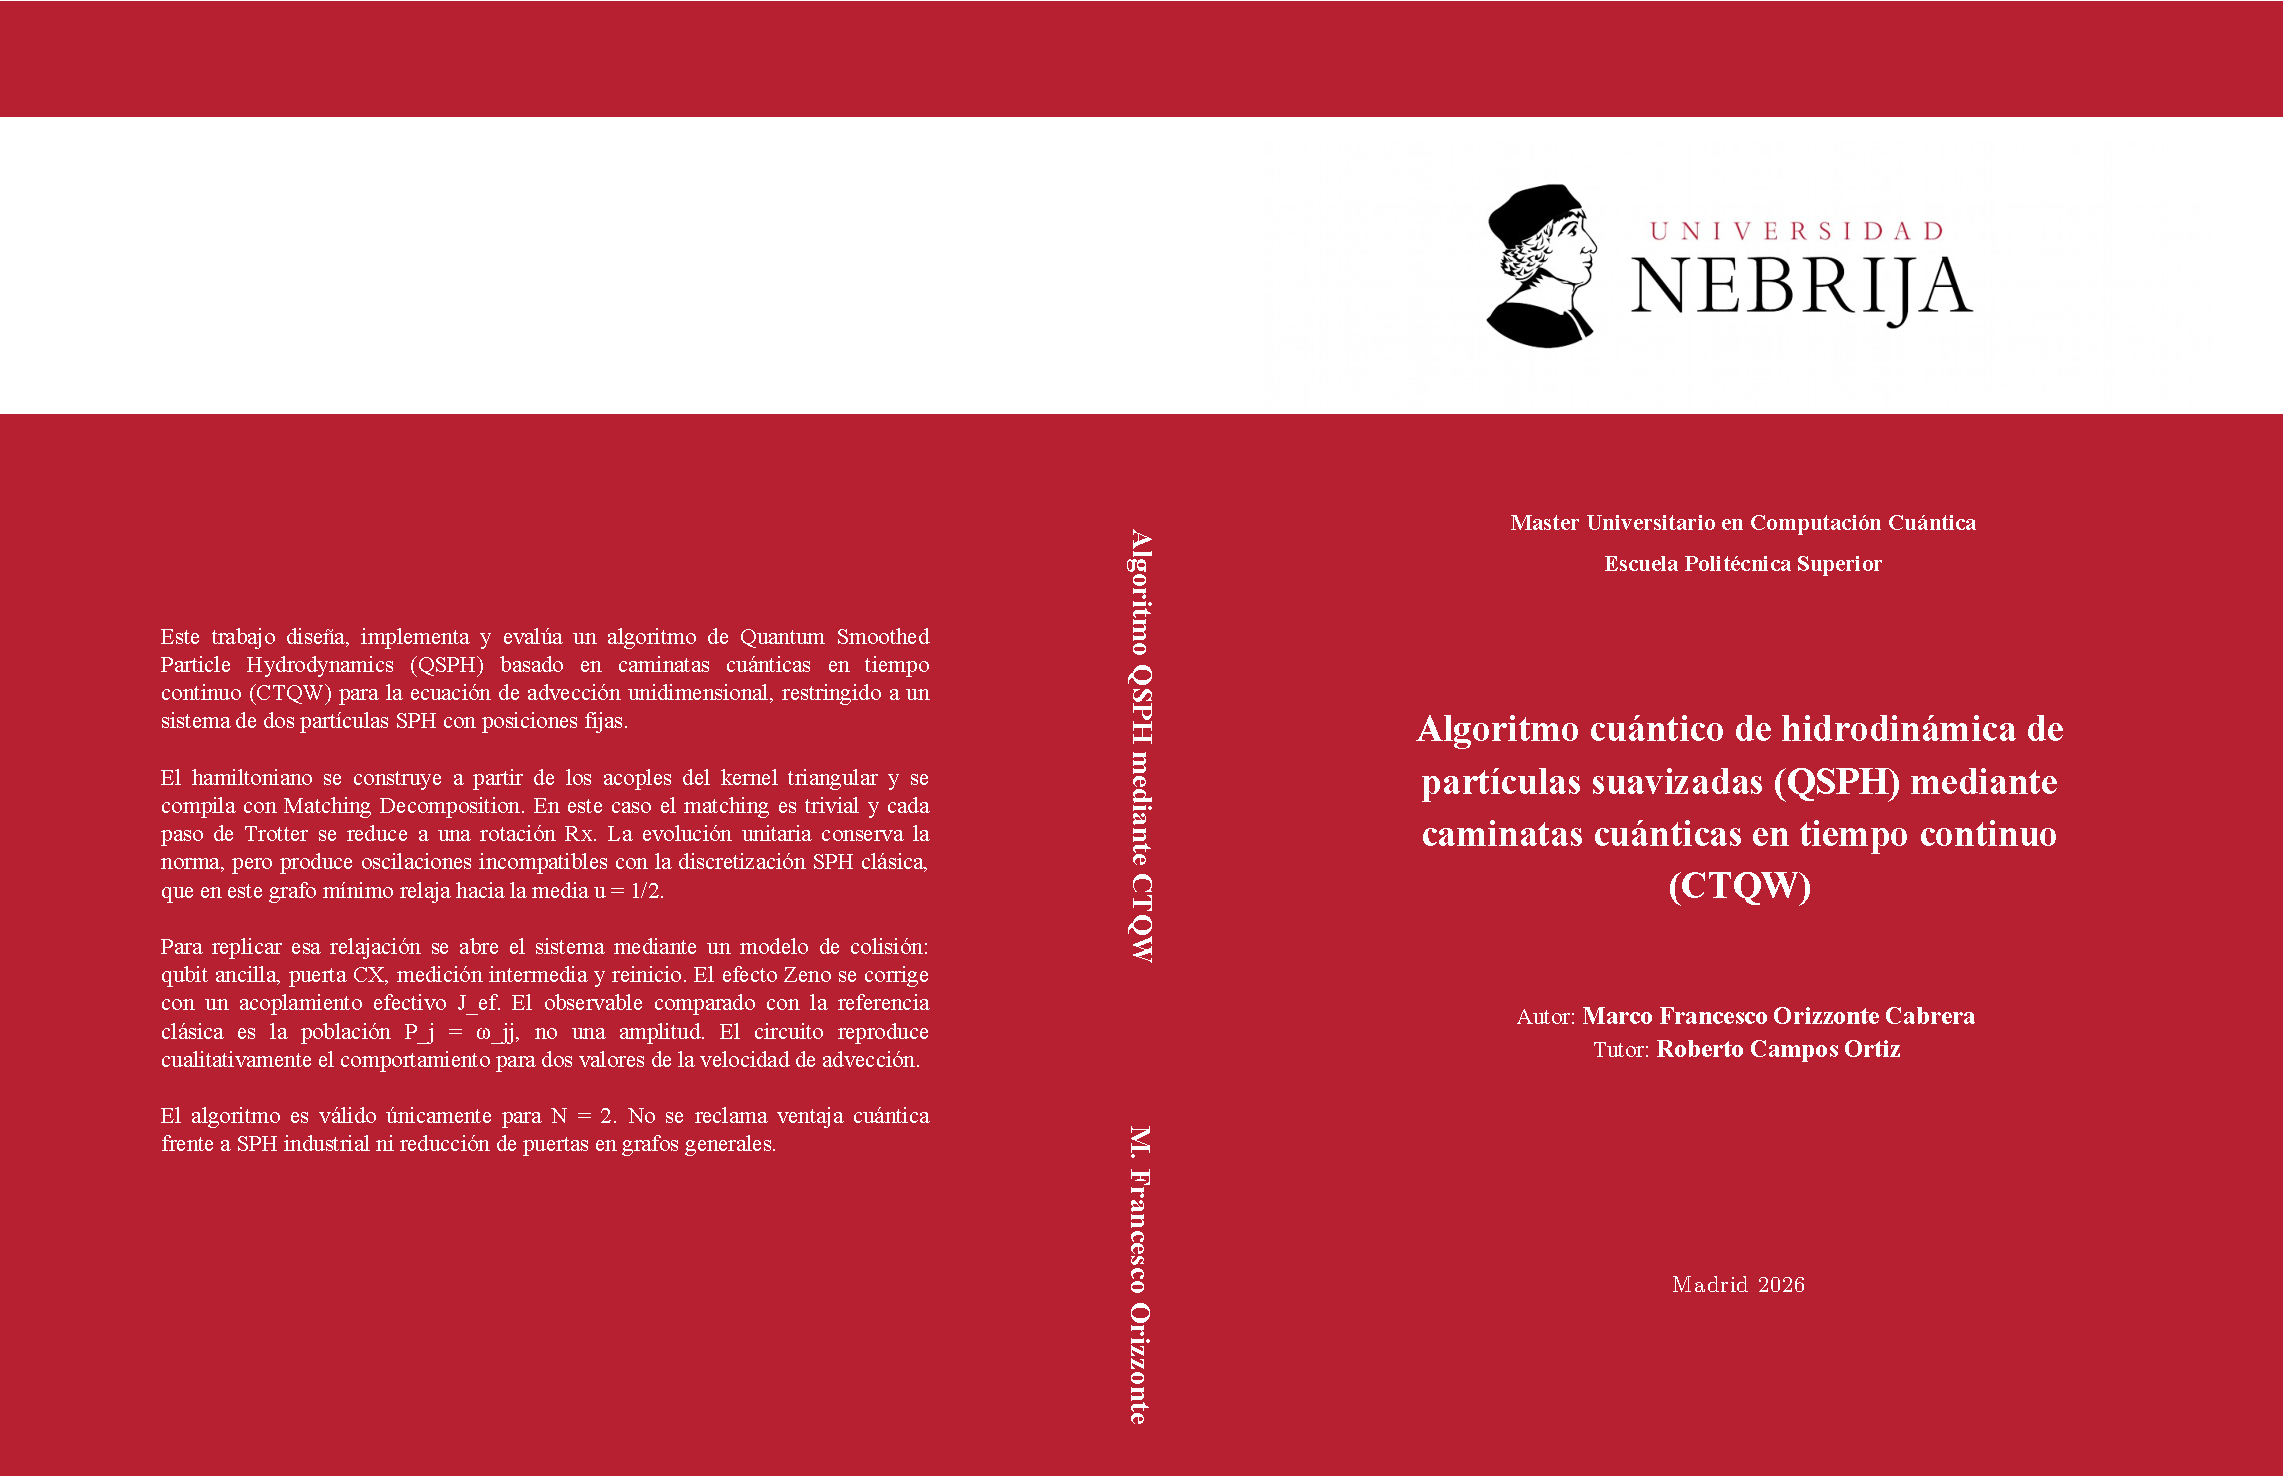
\includepdf[pages=-,fitpaper=true]{cover.pdf}

% ─── PÁGINAS PRELIMINARES (sin numeración) ────────────────────────────────────
\frontmatter
\pagestyle{fancy}

% 1) Hoja en blanco tras la portada.
\hojablanca

% 2) Dedicatoria (cursiva, centrada a la derecha, fuera del índice).
% ─── DEDICATORIA ─────────────────────────────────────────────────────────────
% Página sin numeración, sin cabecera/pie y fuera del índice general.
\thispagestyle{empty}
\vspace*{\fill}
\begin{flushright}
\itshape

A mi hermana, mis padres, abuelos y tíos\\
Los seres más queridos de mi vida\\
A compañera de vida, quien amo incondicionalmente\\
Y como siempre, a mis hermanos de cuatro patas en cielo y tierra\\

%\medskip
%\normalfont\upshape
\end{flushright}
\vspace*{\fill}
\clearpage


% 3) Hoja en blanco tras la dedicatoria.
\hojablanca

% 4) Resumen / Abstract / Agradecimientos (consecutivos, sin blancos entre ellos).
\chapter*{Resumen}
Este trabajo diseña, implementa y evalúa un algoritmo de Quantum Smoothed Particle Hydrodynamics (QSPH) basado en caminatas cuánticas en tiempo continuo (CTQW) para la ecuación de advección unidimensional, restringido a un sistema de dos partículas SPH con posiciones fijas. El hamiltoniano se construye a partir de los acoples del kernel triangular y se compila con Matching Decomposition; en este trabajo el matching es trivial y cada paso de Trotter se reduce a una rotación $R_x$. Se muestra que la evolución unitaria conserva la norma y produce oscilaciones incompatibles con la discretización SPH clásica, la cual, en este grafo mínimo, relaja hacia la media $u=1/2$. Para copiar esa relajación se abre el sistema mediante un modelo de colisión (qubit ancilla, puerta CX, medición intermedia y reinicio) y se corrige el efecto Zeno con un acoplamiento efectivo $J_{\mathrm{eff}}$. El observable comparado con la referencia clásica es la población $P_j=\rho_{jj}$, no una amplitud. El circuito reproduce cualitativamente para dos valores de la velocidad de advección. El algoritmo se considera válido únicamente para $N=2$; no se reclama ventaja cuántica frente a SPH industrial ni la reducción de puertas en grafos generales.

% Abstract
\chapter*{Abstract}
This work, implements and evaluates a Quantum Smoothed Particle Hydrodynamics (QSPH) algorithm based on continuous-time quantum walks (CTQW) for the one-dimensional advection equation, restricted to two SPH particles with fixed positions. The Hamiltonian is built from the couplings of a triangular kernel and compiled with Matching Decomposition; for this scenario the matching is trivial and each Trotter step reduces to an $R_x$ rotation. Unitary evolution conserves the norm and yields oscillations that disagree with the classical SPH behavior, which on this minimal graph relaxes to the mean $u=1/2$. That relaxation is reproduced by opening the system with a collision model (ancilla qubit, CX gate, mid-circuit measurement and reset) and by correcting the quantum Zeno effect with an effective coupling $J_{\mathrm{eff}}$. The observable compared with the classical reference is the population $P_j=\rho_{jj}$, not an amplitude. The circuit matches qualitatively for two advection speeds. The algorithm is validated only for $N=2$; no quantum advantage over industrial SPH, and no CX-count reduction for general graphs, is claimed.

% Agradecimientos
\chapter*{Agradecimientos}
Me gustaría citar unas palabras de un científico muy reconocido en este campo, ``I don’t have to know an answer. I don’t feel frightened by not knowing things, by being lost in the mysterious universe without having any purpose — which is the way it really is, as far as I can tell. Possibly. It doesn’t frighten me.'', Richard Feynman. 

Este trabajo refleja una idea abstracta, de esas que vienen como una corriente de aire refrescante que peina el cabello, más lindo que tener ideas así es el hecho de perseguirlas, de ser capaz de atraparlas y no soltar hasta averiguar más. Para poder llevar a acabo un trabajo así hace falta tener la suerte de no tener más preocupaciones. De evadir el estrés del día a día y estar en una paz tal que nos sea posible disfrutar de esa brisa. Por estas razones doy gracias a mis padres, por darme una oportunidad de disfrutar de la brisa, a pesar de nunca tener una respuesta clara. 

En este camino no voy solo, por tan lejos de nuestra tierra estemos, tengo siempre alguien a mi lado, mi amada Beatriz, la persona con la cual puedo discutir mis ideas y no sentirme incomprendido, la persona con la cual puedo disfrutar de aquellas ideas, la persona a la que ansió ver y contar todo lo nuevo y escuchar cosas maravillosas de otras áreas. La persona la cual siempre me pone los pies en la tierra y saca mi lado más humilde y solidario. 

Y durante este camino, siempre tengo en mente a un ser que crece con una rapidez que hace que mi tiempo pase en un parpadeo. Mi hermana Gia, a la que amo con mi corazón. Durante este trabajo hemos vivido momentos inolvidables y risas incontables, gracias por ser el ser de luz, alegre y llena de amor que siempre me saca una sonrisa.

Para iniciar la lectura de esta brisa maravillosa tengo que mencionar a mis compañeros de cuatro patas, que, tanto en cielo como en tierra, están allí siempre con algo nuevo para hacer, los cuales demuestran que no es necesario tener un abecedario para amar. 

% 5) Hoja en blanco tras los agradecimientos.
\hojablanca

% 6) Estructura de la tesis + Repositorio de código (juntos, fuera del índice).
% ─── ESTRUCTURA DE LA TESIS Y REPOSITORIO ─────────────────────────────────────
% Secciones no numeradas, fuera del índice general (sin \addcontentsline).
% Ambas secciones comparten la misma página, con estilo fancy (numerada).

\section*{Estructura de la tesis}
\noindent Esta memoria se organiza en siete capítulos. El \textbf{Capítulo~1} introduce la motivación del proyecto y la transición desde la simulación clásica de fluidos hacia un modelo cuántico. El \textbf{Capítulo~2} recoge los objetivos, general y específicos, que guían el trabajo. El \textbf{Capítulo~3} desarrolla el marco teórico y el estado del arte: la comparación entre métodos basados en malla y SPH, la ecuación de advección unidimensional, la formulación SPH y las caminatas cuánticas en tiempo continuo (CTQW). El \textbf{Capítulo~4} presenta la metodología, incluyendo la analogía con CTQW, la construcción del Hamiltoniano y la codificación del estado físico. El \textbf{Capítulo~5} describe el diseño e implementación del circuito cuántico, describiendo la descomposición de emparejamiento, la introducción de sistemas abiertos mediante un qubit ancilla y la compensación del efecto Zeno. El \textbf{Capítulo~6} expone los resultados y su discusión para distintas velocidades de advección. Por último, el \textbf{Capítulo~7} recoge las conclusiones y las líneas de trabajo futuro.
\bigskip

\section*{Repositorio de código fuente}
\noindent El código fuente, la memoria en \LaTeX{} y el PDF compilado se encuentran disponibles en un repositorio público de GitHub:
\begin{center}
\href{https://github.com/afroomg/TFM_FrancescoOrizzonte}{\url{https://github.com/afroomg/TFM_FrancescoOrizzonte}}
\end{center}

\noindent El repositorio está estructurado de forma que tanto el código del algoritmo como la memoria pueden reproducirse siguiendo las instrucciones del \texttt{README}. Incluye un entorno de ejecución y un \textit{Makefile} para compilar la documentación y obtener el PDF sin dependencias manuales adicionales.

\medskip\noindent
Conviene aclarar que en esta memoria \textbf{no se incluyen fragmentos de código} (\textit{snippets}). El foco del trabajo es el análisis del algoritmo ---su formulación, las herramientas matemáticas subyacentes y las ecuaciones primordiales que gobiernan la dinámica--- y no los detalles de su implementación. La explicación se centra por tanto en el comportamiento del algoritmo, en el diseño del circuito cuántico y en la interpretación física de los resultados, mientras que el código, debidamente documentado, queda alojado en el repositorio para su consulta y reproducción.


% 7) Hoja en blanco tras estructura/repositorio.
\hojablanca

% 8) Índices.
\tableofcontents
\listoffigures

% 9) Hoja en blanco antes de entrar al cuerpo principal.
\hojablanca

% ─── CUERPO PRINCIPAL ─────────────────────────────────────────────────────────
\mainmatter
\pagestyle{fancy}

% chapters/cap1_introduccion/cap1.tex

\chapter{Introducción y Motivación}

\section{La dinámica de fluidos computacional y sus límites}

La dinámica de fluidos computacional (CFD) es la disciplina que permite resolver de forma numérica las ecuaciones de Navier-Stokes para describir el movimiento de fluidos \cite{Raman2018CFDReview}. Históricamente ligada a la industria aeroespacial, hoy es una herramienta transversal crítica en diversas áreas de la ciencia y la ingeniería. Sus aplicaciones abarcan desde la meteorología y el clima, para predecir la dispersión de contaminantes \cite{Pantusheva2022PollutionCFD}; pasando por la aerodinámica en la industria automotriz y aeroespacial para la optimización de perfiles alares \cite{Slotnick2014CFDV2030}; hasta llegar a la biomedicina, donde simula complejas interacciones en la hemodinámica de arterias y ventrículos \cite{Toma2017SPHBiomedical}. 

A pesar de su éxito, la CFD clásica se enfrenta a un severo cuello de botella. Tanto los métodos basados en malla como los enfoques sin malla como \emph{Smoothed Particle Hydrodynamics} (SPH) exigen recursos masivos para evaluar las interacciones físicas a medida que aumenta la resolución. Aunque herramientas como SPH son excelentes para manejar grandes deformaciones sin necesidad de remallar, la carga combinatoria de buscar partículas vecinas en cada iteración sigue planteando tiempos de ejecución muy restrictivos a nivel industrial. Este TFM no resuelve ese cuello de botella, se busca estudiar el caso mínimo de dos partículas SPH fijas.

Para ilustrar la versatilidad de estas simulaciones, la figura \ref{fig:particles_combined} muestra la aplicabilidad del método de mallas y de la formulación SPH.

\begin{figure}[htbp]
    \centering
    % Primera subfigura (Cráneo)
    \begin{subfigure}[b]{0.48\textwidth}
        \centering
        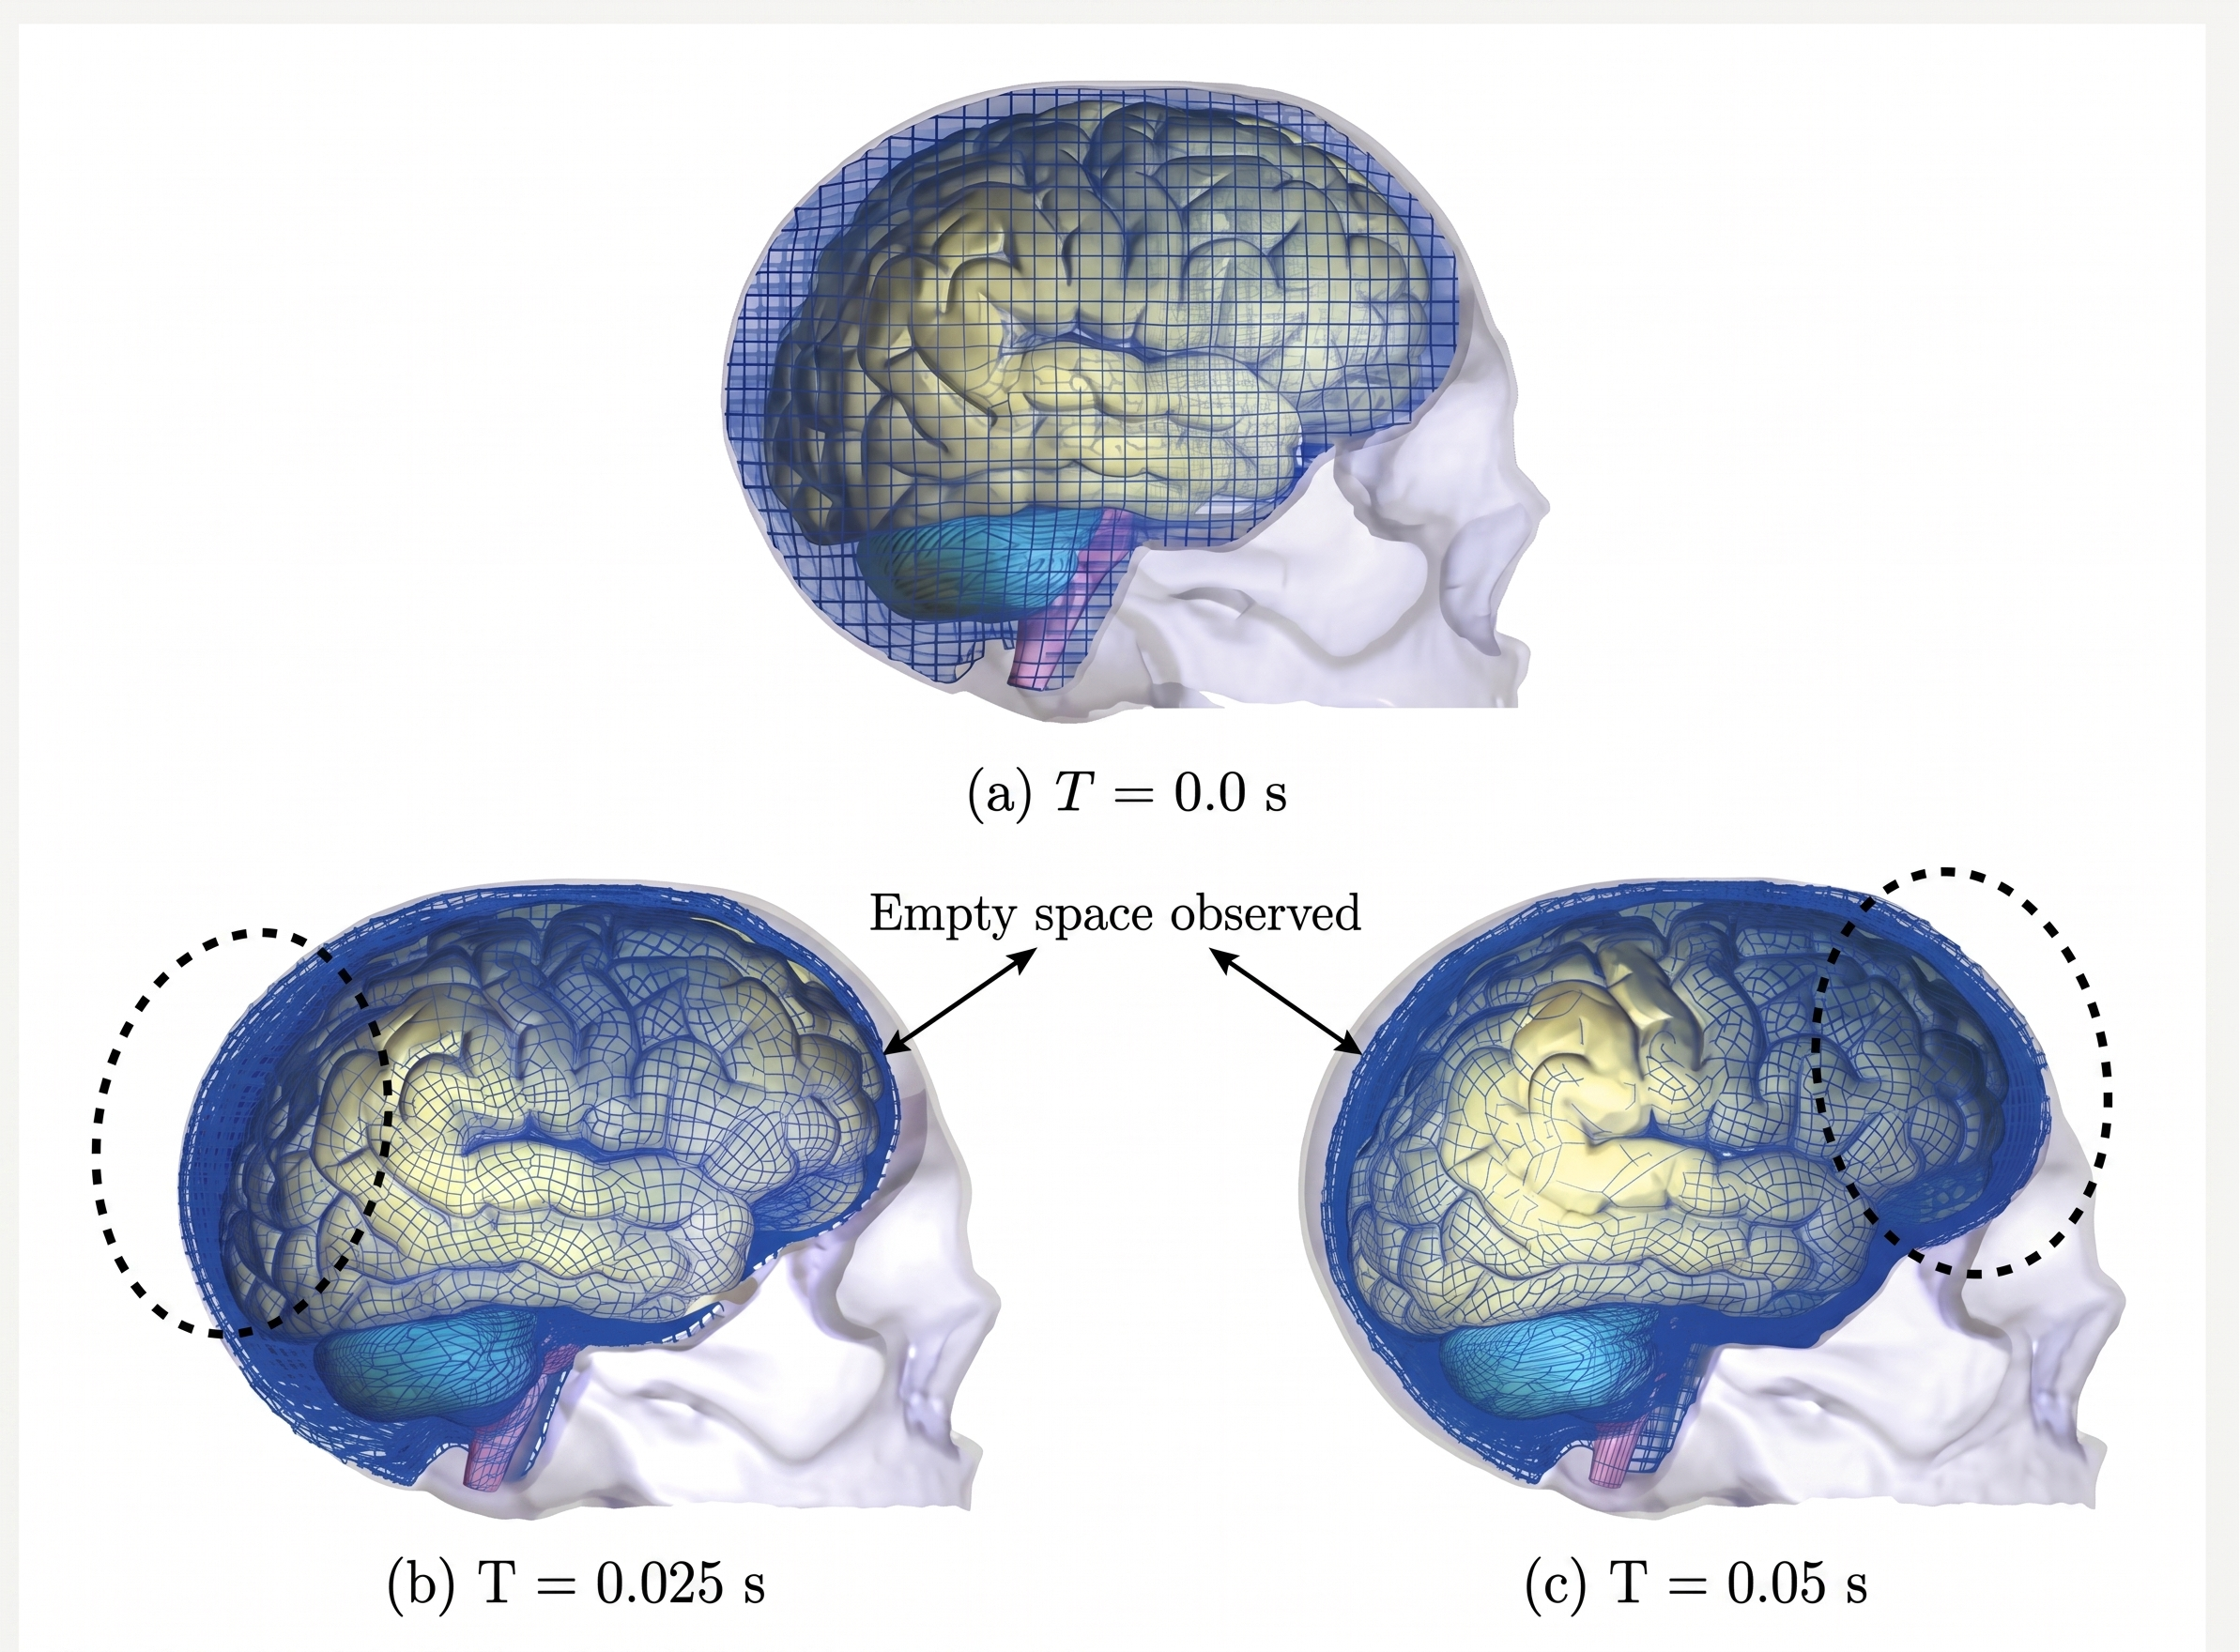
\includegraphics[width=\textwidth]{chapters/cap1_introduccion/img/craneo.png}
        \caption{Simulación de aceleración y desaceleración, mostrando la hemodinámica dentro del cráneo. Adaptado de \cite{Toma2017SPHBiomedical}.}
        \label{fig:craneo_sph}
    \end{subfigure}
    \hfill
    % Segunda subfigura (Parque eólico)
    \begin{subfigure}[b]{0.48\textwidth}
        \centering
        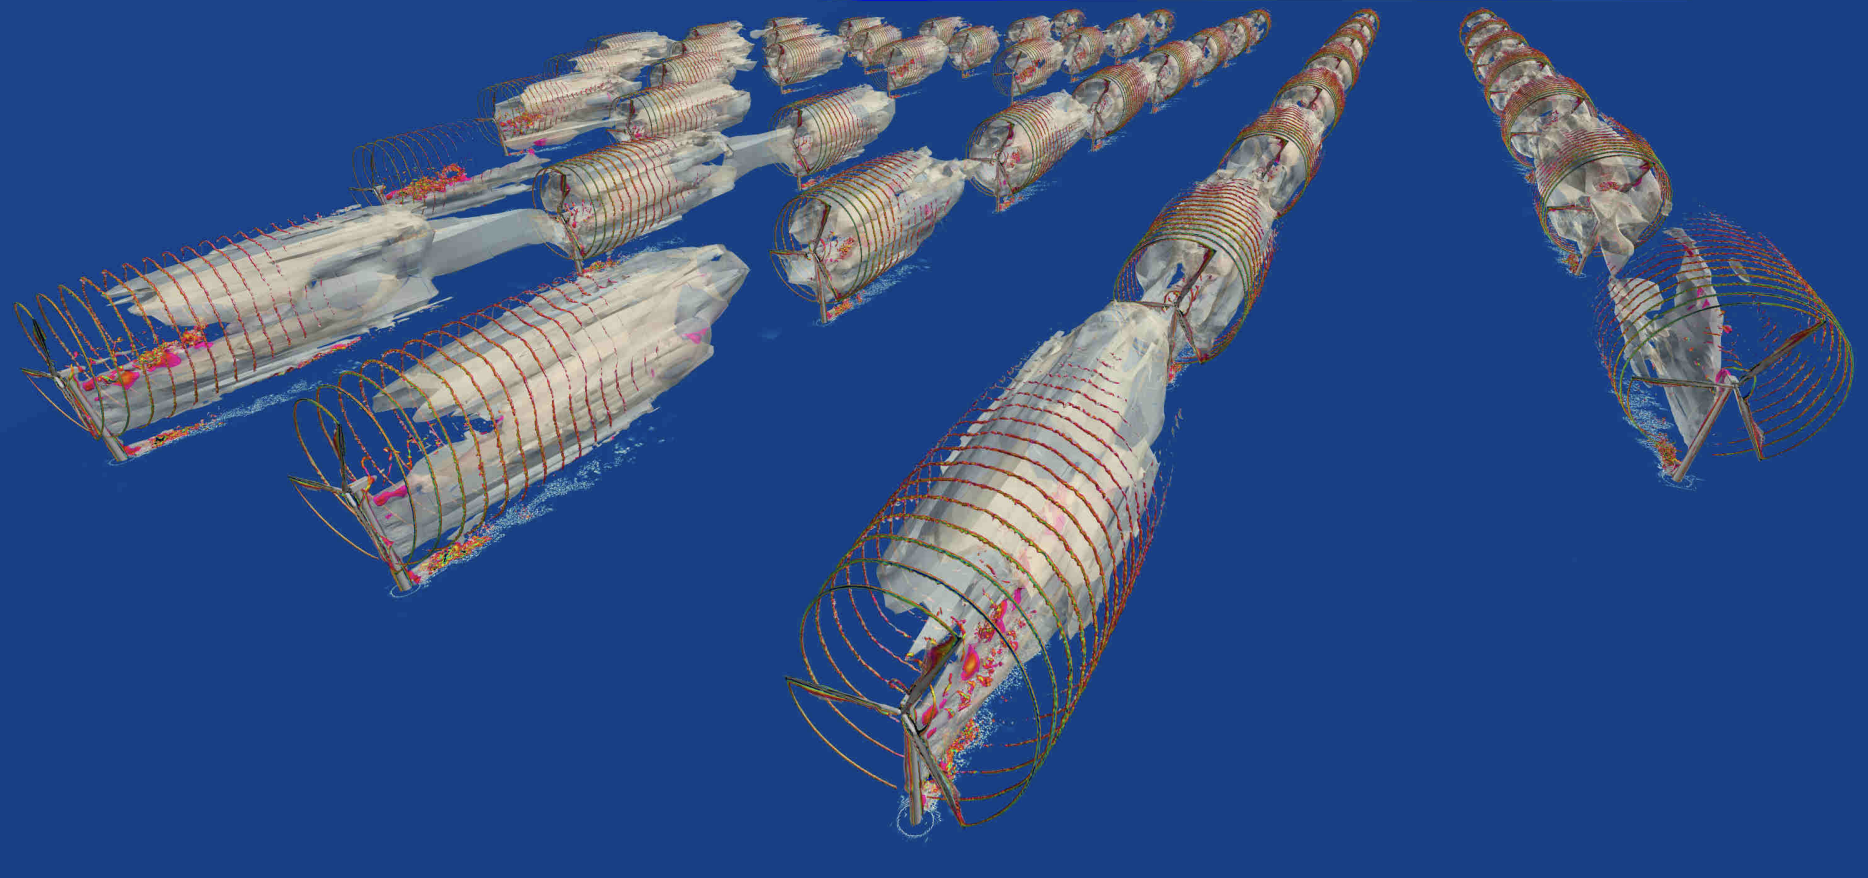
\includegraphics[width=\textwidth]{chapters/cap1_introduccion/img/turbine.png}
        \caption{Estructuras de estela en el parque eólico Lillgrund. Adaptado de \cite{Kirby2018}.}
        \label{fig:windfarm_wake}
    \end{subfigure}
    
    \caption{Ejemplos de simulación en dinámica de fluidos. (a) Hemodinámica craneal, adaptado de Toma (2017). (b) Estelas en el parque eólico Lillgrund, adaptado de Kirby et al. (2018).}
    \label{fig:particles_combined}
\end{figure}

\section{Paso de computación clásica a un modelo cuántico}

La computación cuántica surge como una vía prometedora para superar estas barreras algorítmicas clásicas. Más allá del rigor matemático, este proyecto nace de una intuición abstracta sobre la naturaleza del transporte. En el método de partículas (SPH), el fluido se discretiza en nodos que interactúan según un kernel de suavizado. Si representamos esta estructura como un grafo de interacciones, el flujo del fluido puede interpretarse como el recorrido de información a través de dicho grafo. Existe una analogía profunda entre cómo un fluido físico se desplaza y cómo la amplitud de probabilidad cuántica explora un espacio de estados en un grafo.

Investigaciones recientes han propuesto algoritmos de \emph{Quantum Smoothed Particle Hydrodynamics} (QSPH) para mapear la ecuación de advección clásica a circuitos cuánticos, destacando los notables trabajos de Au-Yeung, Williams et al. \cite{auyeung2024, auyeung2025}. Si bien el presente documento se fundamenta en gran medida en su exhaustivo estudio basado en Caminatas Cuánticas en Tiempo Discreto (DTQW), dicho enfoque presenta ciertas limitaciones, como la necesidad de registros auxiliares de moneda (\emph{coin register}) y la aparición de algunos términos adicionales en el cálculo. Por ello, nuestra metodología de implementación busca explorar un camino diferente para evaluar si es posible alcanzar una solución más directa o eficiente para el mismo problema físico.

\section{Justificación del proyecto}

La motivación principal de este proyecto es buscar una alternativa para determinar un primer paso hacía otro camino en busca de alguna mejora con respecto al estado del arte actual en QSPH, implementando Caminatas Cuánticas en Tiempo Continuo (CTQW). En este paradigma, el hamiltoniano del sistema puede construirse directamente a partir de la matriz de adyacencia de los coeficientes del kernel SPH, lo que podría simplificar la formulación de la evolución del fluido sin requerir registros adicionales.

El interés en explorar esta alternativa radica en un problema crítico de la industria, debido a que la dinámica de fluidos computacional (CFD) de alta fidelidad representa una de las mayores cargas de trabajo en los superordenadores modernos a nivel global \cite{Karp2024CFDMSA}. Por ejemplo, simulaciones recientes de dinámica de fluidos en el superordenador de exaescala \textit{Frontier} (Oak Ridge National Laboratory, EE. UU.) han requerido paralelizar billones de puntos de malla y miles de GPUs durante horas para resolver problemas aeroespaciales y energéticos, acaparando una inmensa fracción del consumo energético y de los ciclos de CPU/GPU de estas instalaciones \cite{OakRidge2025FrontierCFD}.

Dada la altísima relevancia de aplicaciones como el diseño aeroespacial, la optimización automotriz y la biomedicina, acelerar estas dinámicas es una necesidad tecnológica urgente. Por tanto, este trabajo investiga si un CTQW, compilado con \emph{Matching Decomposition}, puede reproducir la discretización SPH \eqref{eq:sph_advection_discrete} en el dímero de dos partículas fijas. \emph{Matching Decomposition} se adopta como método de compilación \cite{matching2026}; en $N=2$ no se demuestra reducción de profundidad ni alivio de la demanda CFD en hardware NISQ. El criterio de éxito es la correspondencia cualitativa con la ecuación \eqref{eq:sph_advection_discrete}, no una aceleración industrial.

% chapters/cap2_objetivos/cap2.tex

\chapter{Objetivos}
\label{ch:objetivos}

El desarrollo de este trabajo fin de máster se articula en torno a un objetivo general que define el propósito y alcance de la investigación, del cual se derivan una serie de objetivos específicos que trazan la hoja de ruta metodológica y técnica para su consecución.

\section{Objetivo general}

El objetivo principal de este trabajo es diseñar, implementar y evaluar un algoritmo cuántico basado en caminatas cuánticas en tiempo continuo (CTQW) para la resolución de la ecuación de advección unidimensional, para un sistema de dos partículas SPH con posiciones fijas. Se busca analizar cómo evoluciona en el tiempo una cantidad advectada a partir de unas condiciones iniciales dadas, evaluando la viabilidad y fidelidad física de este enfoque frente a la discretización SPH clásica \eqref{eq:sph_advection_discrete} en el mismo escenario de dos partículas.

\section{Objetivos específicos}

Para alcanzar el objetivo general propuesto, se plantean los siguientes objetivos específicos:

\begin{enumerate}
    \item \textbf{Estudio y adaptación del formalismo SPH:} Analizar en profundidad el método clásico de \emph{Smoothed Particle Hydrodynamics} (SPH) y desarrollar la formulación matemática necesaria para transicionar de este modelo clásico a un SPH cuántico, garantizando la generación de estados cuánticos válidos y representativos de las propiedades del fluido.
    
    \item \textbf{Formulación del algoritmo basado en CTQW:} Establecer el marco teórico y operativo para mapear la dinámica del fluido utilizando caminatas cuánticas en tiempo continuo, construyendo el hamiltoniano del sistema a partir de la matriz de adyacencia del grafo de interacción de partículas.
    
    \item \textbf{Compilación del hamiltoniano:} Aplicar \emph{Matching Decomposition} \cite{matching2026} para implementar $e^{-iHt}$ sin descomposición de Pauli. En $N=2$ el \emph{matching} es trivial y el bloque es una $R_x$; no se toma como objetivo demostrar la reducción de $CX$ o de profundidad reportada por esos autores en grafos generales.
    
    \item \textbf{Implementación computacional en Qiskit:} Programar y simular el circuito cuántico resultante utilizando Python y el framework Qiskit, integrando el método de \emph{Matching Decomposition} para la ejecución de la dinámica de la caminata cuántica en simuladores.
    
    \item \textbf{Codificación y lectura:} Preparar el estado mediante \emph{Amplitude Encoding} del escalar inicial y leer las poblaciones $P_j = \rho_{jj}$, identificadas con $u_j$ al comparar con \eqref{eq:sph_advection_discrete}. No se evalúa \emph{Quantum Amplitude Estimation} ni se reconstruye la amplitud compleja.
    
    \item \textbf{Sistema cerrado frente a abierto:} Contrastar el CTQW unitario (oscilaciones) con un mapa abierto realizado como modelo de colisión (ancilla, $CX$, medida y reinicio), más la corrección de Zeno, para reproducir la relajación de \eqref{eq:sph_advection_discrete} en el dímero.
\end{enumerate}

% chapters/cap3_marcoteorico/cap3.tex

\chapter{Marco Teórico y Estado del Arte}
\label{ch:marco_teorico}

Para comprender la propuesta de este trabajo, es necesario establecer las bases físicas y computacionales que rigen el problema que se quiere afrontar. Este capítulo da una breve descripción desde los fundamentos clásicos de la dinámica de fluidos computacional (CFD), haremos más hincapié en la formulación SPH ya que es el foco principal, veremos el significado físico de la ecuación de advección y bases para comprender el apoyo de las caminatas cuánticas de tiempo continuo (CTQW).

\section{Simulación de fluidos: Malla vs. SPH}

La mecánica de fluidos computacional tiene dos formulaciones con enfoques diferentes, el primero es el enfoque euleriano, de malla el cual ilustra el fluido desde fuera y el enfoque lagrangiano, de partículas, el cual intenta describir el fluido por la interacción de las partículas. Conocer sus límites resulta imperativo, pues sus cuellos de botella clásicos alimentan la búsqueda de aceleración cuántica.

\subsection*{Métodos basados en malla (eulerianos)}
En los métodos de malla —FVM, FEM, FDM— el dominio se escinde en celdas fijas a través de las cuales las propiedades del fluido migran en el tiempo.

\begin{itemize}
    \item \textbf{Fortalezas:} Constituyen el estándar de la industria aeronáutica y automotriz. Gozan de sólidos fundamentos matemáticos, conservación estricta de flujos y precisión geométrica insuperable para configuraciones estables.
    \item \textbf{Fragilidades:} Ante cambios topológicos —superficies libres, deformaciones extremas o interacción fluido-estructura— exigen remallado dinámico, lo que encarece el cálculo hasta volverlo inviable y propaga inestabilidades numéricas.
\end{itemize}

\subsection*{Métodos de partículas: SPH (lagrangianos)}
El \emph{Smoothed Particle Hydrodynamics} renuncia a la malla. El fluido se atomiza en partículas autónomas que portan masa y presión, y el sistema evoluciona por interacciones vecinales.

\begin{itemize}
    \item \textbf{Fortalezas:} Captura con naturalidad salpicaduras, roturas e impactos violentos. Al suprimir la fase de mallado —que en proyectos industriales consume semanas—, el tiempo de preparación se reduce drásticamente.
    \item \textbf{Fragilidades:} Las condiciones de contorno resultan matemáticamente esquivas, y la resolución fina exige masas de partículas que empalidecen la parsimonia de los métodos de malla.
\end{itemize}

\begin{figure}[htbp]
    \centering
    \begin{minipage}[t]{0.48\textwidth}
        \centering
        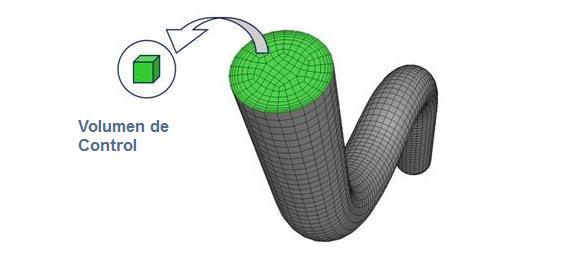
\includegraphics[width=\textwidth]{chapters/cap3_macro/img/malla.jpg}
        \captionof{figure}{Discretización de volumen de control mediante enfoque Euleriano \cite{esss_cfd}.}
        \label{fig:malla}
    \end{minipage}
    \hfill
    \begin{minipage}[t]{0.48\textwidth}
        \centering
        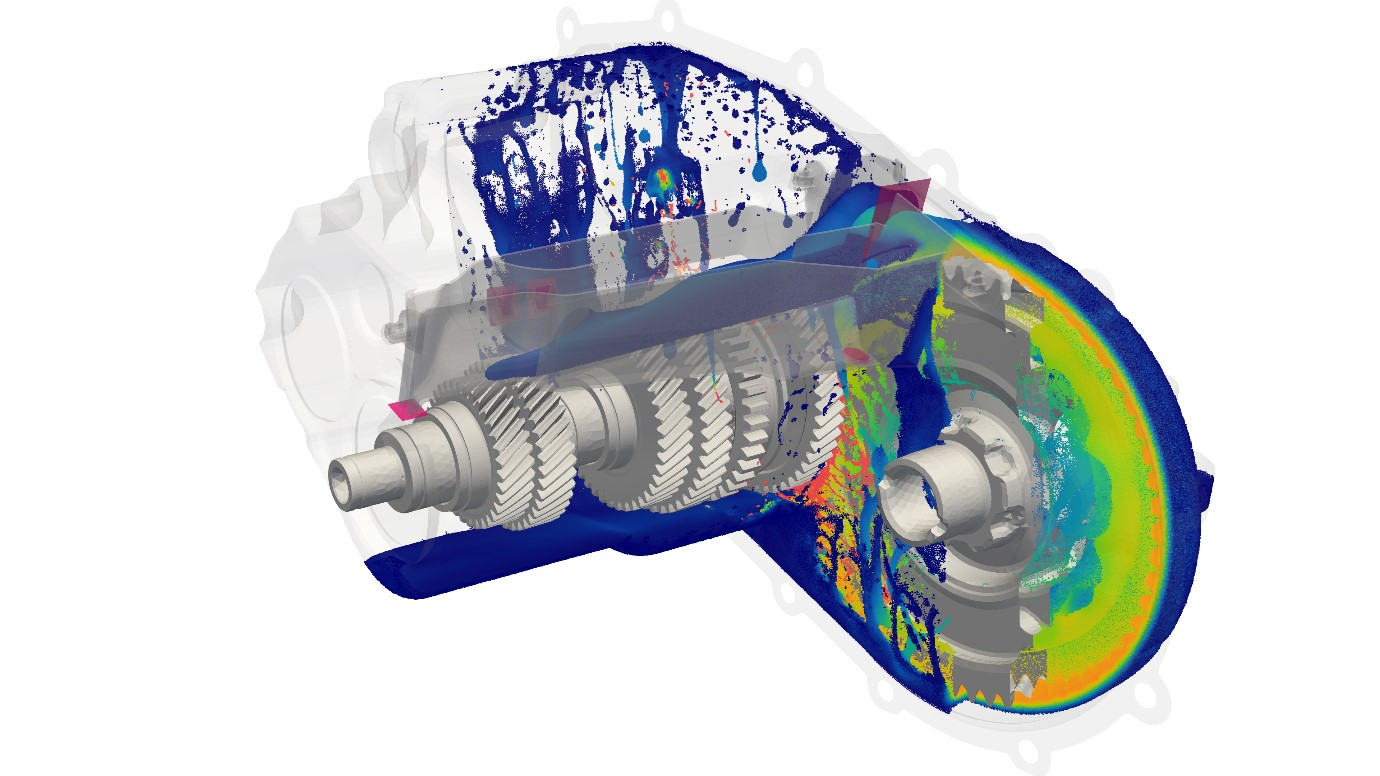
\includegraphics[width=\textwidth]{chapters/cap3_macro/img/sph.jpg}
        \captionof{figure}{Simulación altamente dinámica mediante SPH, sin necesidad de remallado \cite{nextflow_sph_2020}.}
        \label{fig:sph}
    \end{minipage}
\end{figure}


\subsection{Complejidad en métodos de malla}

En la CFD clásica por malla, el cuello de botella es de carácter \textbf{global}: surge al linealizar y resolver los grandes sistemas algebraicos (matrices dispersas) derivados de las ecuaciones de Navier-Stokes. 

Para un dominio 3D discreto con $N$ nodos por dimensión, el número de grados de libertad es $n \sim cN^3$ (donde $c$ es el número de variables por nodo). Un tratamiento directo denso exigiría tiempos inasumibles de $O(n^3) = O(N^9)$. En la práctica, códigos industriales como FUN3D (NASA) o CODA (DLR) emplean métodos iterativos de Krylov (como GMRES) explotando la matriz dispersa. Según el estudio de Wood et al. \cite{Wood2020SLAT} y Wagner \cite{Wagner2021CODASpliss}, el coste temporal por paso de simulación se aproxima a:
\[
C_{\text{Malla}} \sim O(k \cdot N^3)
\]
donde $k$ es el número de iteraciones del solver (dependiente del precondicionador y la física del flujo). Aunque esta complejidad no es matemáticamente exponencial, las exigentes constantes de cálculo, la sincronización de memoria y la resolución de turbulencia hacen que este coste siga siendo un reto masivo de cara a la agenda \textit{CFD Vision 2030} \cite{Slotnick2014CFDV2030}. La resolución de este sistema lineal llega a consumir entre el 50\% y el 90\% del tiempo de simulación \cite{Wood2020SLAT}.


\subsection{Complejidad en SPH}

Para entender de una manera más intuitiva la complejidad del método de SPH se puede consultar la siguiente sección \ref{sec:sph}, en donde se introduce la formulación SPH. Principalmente la complejidad radica en dos etapas, la búsqueda de partículas vecinas con las que una sola interactúa y su posterior procesamiento.

Para un sistema con $M$ partículas, el método más rudimentario consiste en evaluar la interacción directa de cada partícula con todas las demás (\textit{All-pair search}), para comprobar si una determinada partícula está dentro del radio de interacción de otra. Como se describe en \cite{liu2003sph}, esto implica un coste computacional cuadrático $O(M^2)$, inviable para aplicaciones reales. Para evitarlo, se aprovecha el radio de soporte compacto del kernel (denotado como $h$) mediante algoritmos de estructuración espacial, reduciendo drásticamente las interacciones computadas:

\begin{itemize}
    \item \textbf{Búsqueda por Árboles (ej. Octrees):} Estructuran el dominio de forma jerárquica logrando un coste $O(M \log M)$. Son necesarios cuando las partículas poseen longitudes de suavizado ($h$) variables y adaptativas.
    \item \textbf{Listas enlazadas (\textit{Linked-lists}):} En lugar de comparar cada partícula una con otra, se divide el espacio en una cuadrícula y se mide la distancia de una partícula con otra solo si están en la misma celda o si están en celdas vecinas. Esto puede llegar a alcanzar una complejidad teórica óptima de $O(M)$. Pero no es tan eficiente con longitudes de suavizado ($h$) variables.
\end{itemize}

A pesar de que el algoritmo de búsqueda puede optimizarse a niveles de $O(M)$, SPH exige un esfuerzo computacional masivo. La limitación de SPH como vemos no es la acotación de listas de interacciones, sino tres factores físicos y de hardware:

\begin{enumerate}
    \item \textbf{Carga aritmética local:} En SPH 3D, una sola partícula puede interactuar con algunas partículas hasta cientos de vecinos. Para cada par, el procesador debe calcular su respectiva distancia, interpolar el polinomio del kernel $W(r,h)$ y evaluar sus gradientes espaciales para las fuerzas físicas \cite{liu2003sph}. Para simular $M$ partículas, esto significa realizar cientos de millones de operaciones matemáticas por cada instante de tiempo.
    
    \item \textbf{Memoria (\textit{Cache Misses}):} A diferencia de una malla estática donde los datos son contiguos, la naturaleza móvil de las partículas SPH provoca que vecinos físicamente cercanos en el espacio tridimensional estén almacenados en posiciones aleatorias de la memoria RAM. Este acceso desordenado destruye la coherencia de caché. Las CPUs y GPUs desperdician la mayor parte del tiempo esperando a que los datos lleguen de la memoria principal en lugar de realizar cálculos \cite{Staubach2010SPHSystemSimulation}.
    
    \item \textbf{Restricción temporal (Condición CFL):} Para garantizar la estabilidad de la integración numérica, el paso de tiempo $\Delta t$ está limitado por la condición de Courant-Friedrichs-Lewy (CFL). El avance debe ser minúsculo (del orden de microsegundos) para capturar la acústica y el movimiento sin que las partículas crucen a otros dominios repentinamente \cite{Mocz2020SPH}. Esto obliga a calcular repetitivamente toda la búsqueda espacial y la aritmética para las partículas decenas de miles de veces para simular un solo segundo de realidad.
\end{enumerate}

Con esta información podemos ver que, mientras la malla tradicional es limitada en resoluciones algebraicas globales $O(N^3)$ y en cambio el formalismo SPH es limitado localmente. Su barrera no es la complejidad matemática de la búsqueda, sino la inmensa densidad de cálculo combinatorio, el acceso errático a la memoria clásica y la fragmentación temporal. Estos límites clásicos son los que justifican directamente la exploración de otros métodos.


\section{La ecuación de advección unidimensional}
\label{sec:adcevtion}

Es importante para el lector entender el fenómeno físico que este trabajo busca simular. En mecánica de fluidos, la advección se define como el transporte de una cantidad escalar (como la masa, la temperatura o un contaminante) por el movimiento macroscópico o \emph{bulk motion} de un campo de velocidades \cite{leveque2002finite}.

La ecuación de advección es una ecuación diferencial parcial hiperbólica de primer orden que gobierna este transporte. En su forma más fundamental y asumiendo un flujo incompresible en una dimensión ($1D$), la ecuación se expresa como:
\begin{equation}
    \frac{\partial f}{\partial t} + c \frac{\partial f}{\partial x} = 0
    \label{ec: advection}
\end{equation}

donde $f(x,t)$ es la cantidad o propiedad escalar que está siendo advectada, $t$ es el tiempo, $x$ es la coordenada espacial y $c$ representa el campo de velocidad constante del fluido.

El significado físico de esta ecuación radica en la conservación de la propiedad a lo largo del flujo; establece que la tasa de cambio local de $f$ en un punto fijo depende directamente del gradiente espacial de la propiedad y de la velocidad con la que el fluido la arrastra. En el contexto de este trabajo, la resolución de la ecuación de advección 1D es de vital importancia, ya que constituye el problema de referencia más simple para aislar y validar el comportamiento de transporte de nuestro algoritmo cuántico. Con dos nodos fijos, \eqref{eq:sph_advection_discrete} no realiza ese transporte a lo largo de características, ya que se una produce reljación hacia la media.


\section{Formulación SPH y discretización de la advección}
\label{sec:sph}

La base matemática del \textit{Smoothed Particle Hydrodynamics} (SPH) se fundamenta en la teoría de la interpolación a través de la propiedad de filtrado de la función delta de Dirac. Para una función continua arbitraria $f(x)$, esta propiedad establece que el valor de la función en un punto se puede obtener como una integral definida en el dominio $\Omega$:
\begin{equation}
    f(x) = \int_{\Omega} f(y) \delta(x - y) dy
    \label{eq:dirac_property}
\end{equation}
Sin embargo, en el método SPH no se puede trabajar con la singularidad matemática de la delta de Dirac. En su lugar, esta distribución se reemplaza por una función de aproximación conocida como \textit{kernel} de suavizado $W(r, h)$. Este kernel aproxima la función continua mediante:
\begin{equation}
    f(x) \approx \int_{\Omega} f(y) W(x - y, h) dy
    \label{eq:kernel_approximation}
\end{equation}
donde $h$ es la longitud de suavizado (\textit{smoothing length}) que define el radio de soporte compacto del kernel, y $r = |x - y|$ es la distancia entre el punto de interés y sus vecinos. 

El \textit{kernel} es, en esencia, la función geométrica que describe la intensidad de la interacción entre una partícula y su entorno local (véase la figura \ref{fig:kernel_sph}). Al definir el kernel de una forma geométrica conocida, con SPH se logra calcular las derivadas de campos continuos de forma analítica trasladando el operador diferencial a ese kernel, evitando la necesidad de mallas.

\begin{figure}[htbp]
    \centering
    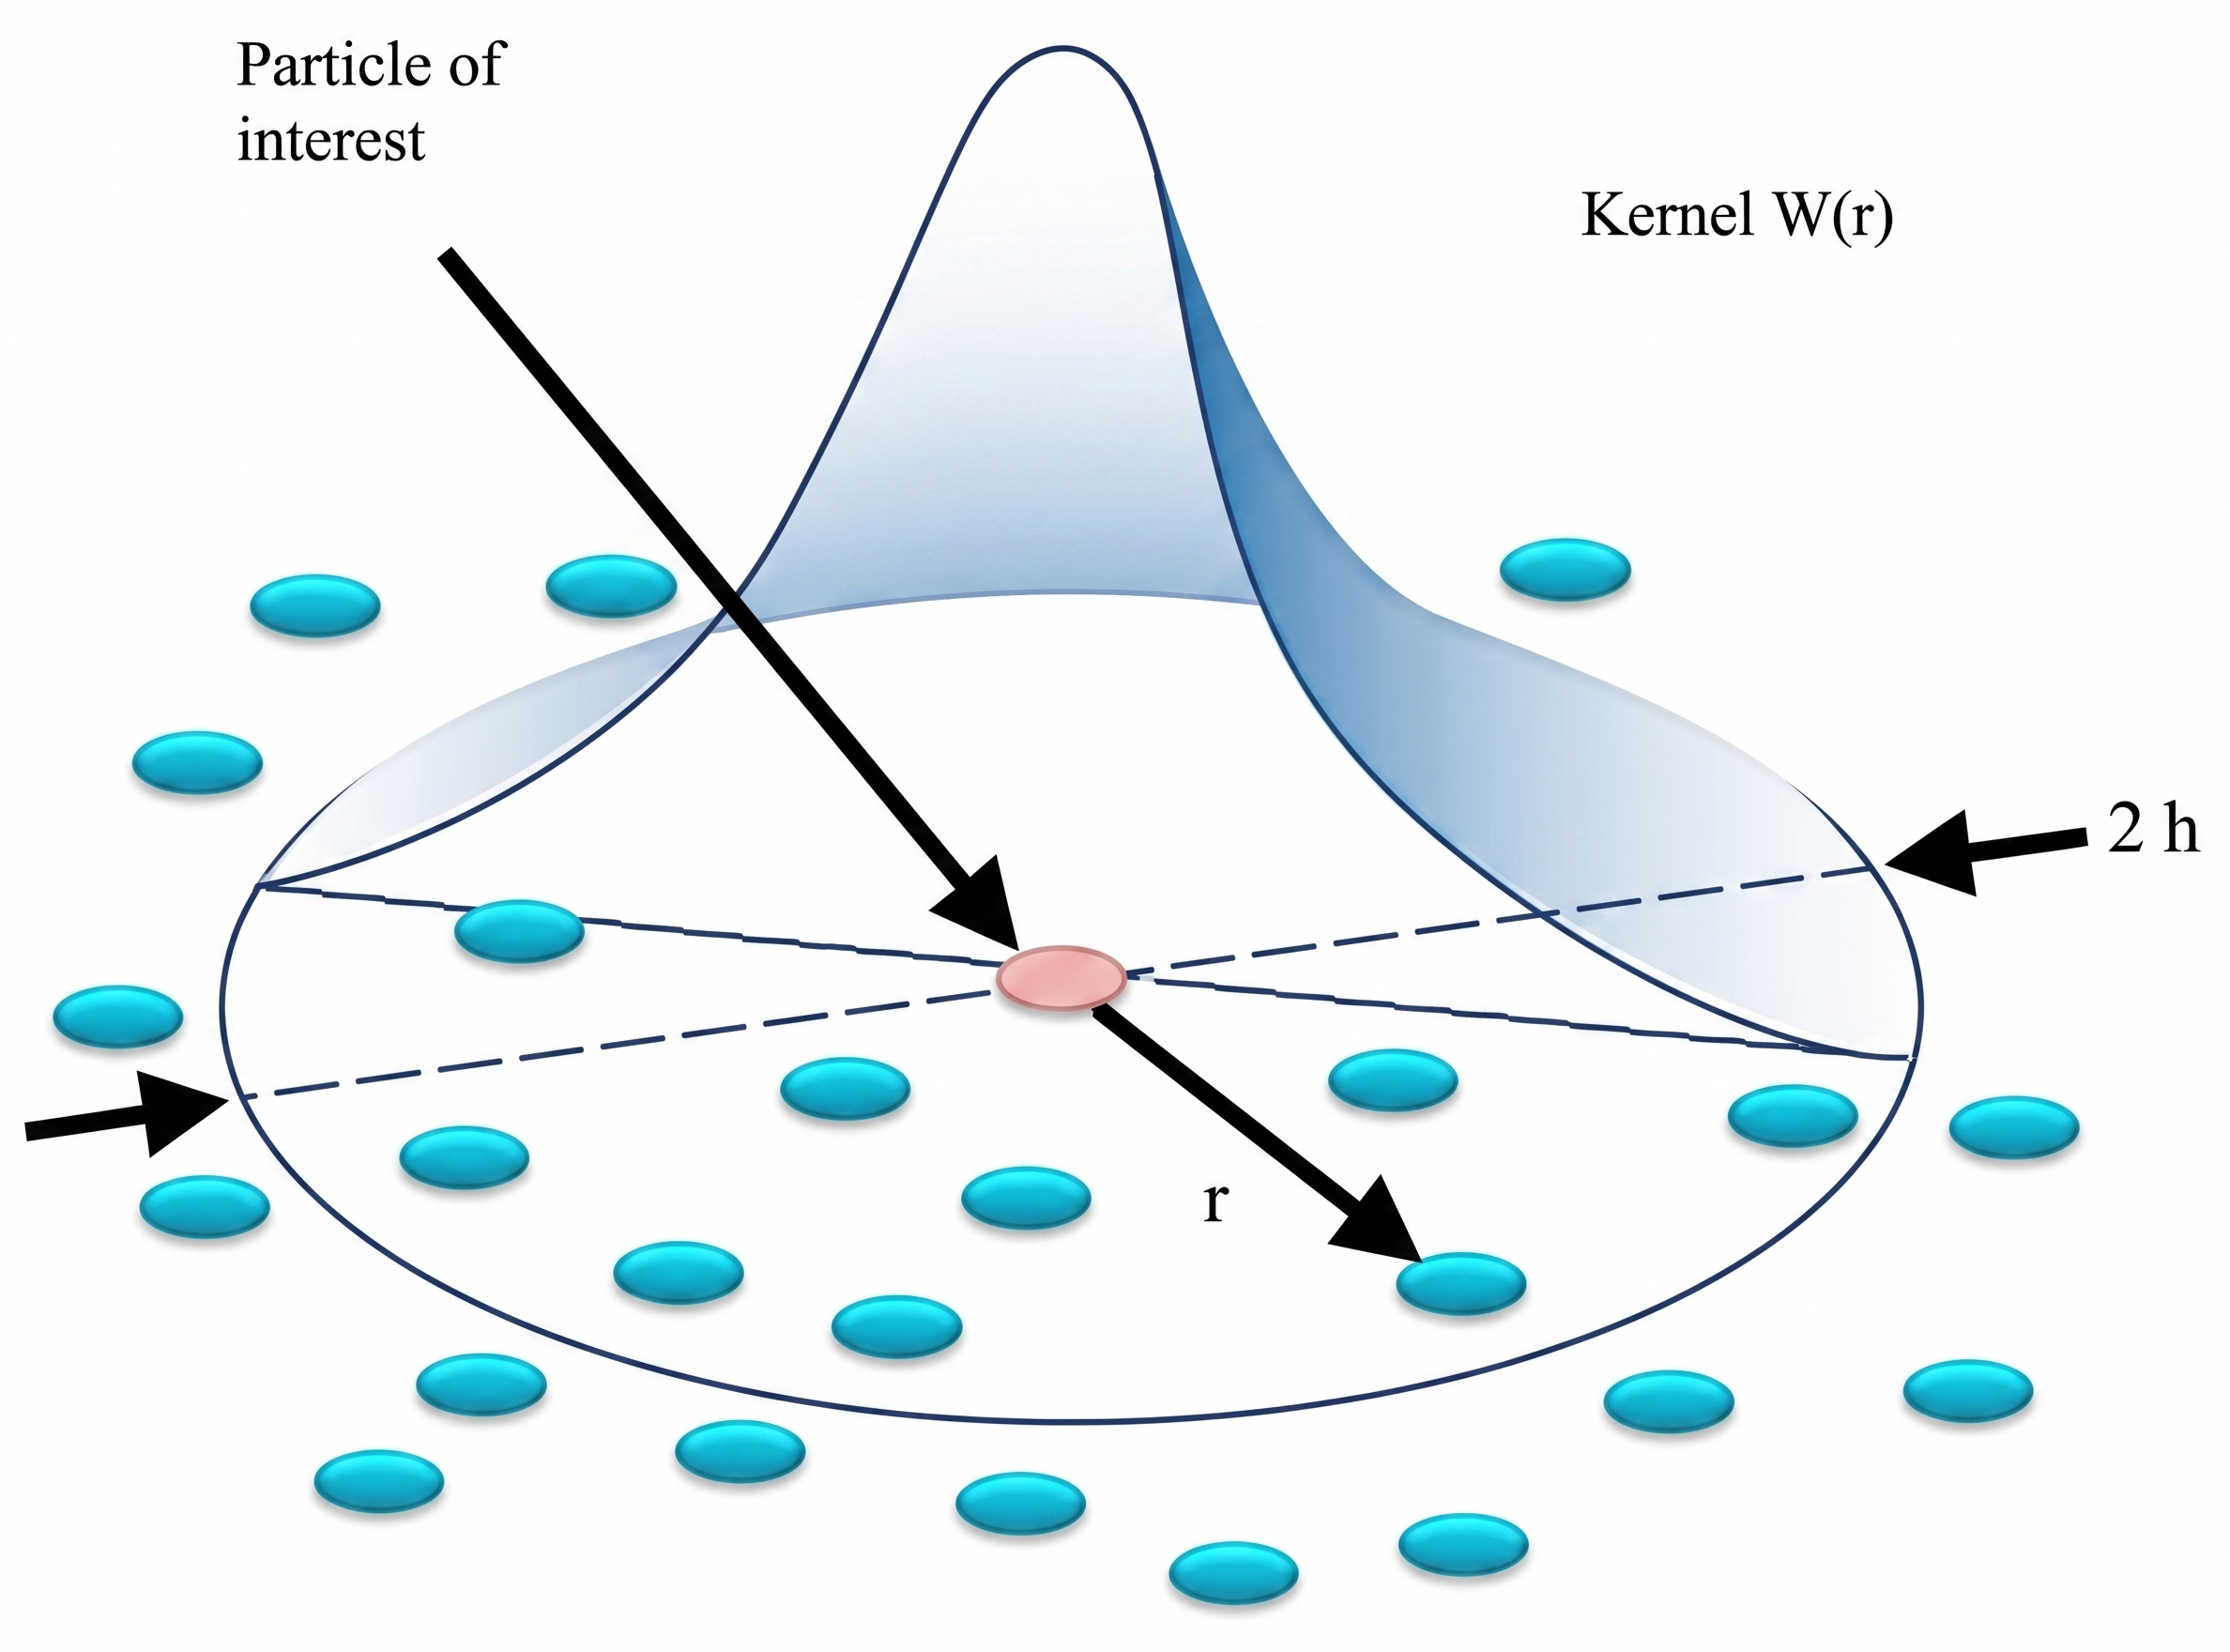
\includegraphics[width=0.6\textwidth]{chapters/cap3_macro/img/kernelsph.png}
    \caption{Representación visual de la función de kernel $W(r, h)$ sobre un sistema de partículas. El parámetro $h$ define el límite del soporte compacto, fuera del cual las interacciones entre partículas se asumen nulas.}
    \label{fig:kernel_sph}
\end{figure}

Al pasar de una integral continua a una sumatoria sobre partículas discretas, el fluido deja de tratarse como un volumen continuo y pasa a representarse como una nube de puntos interactuantes (Figura \ref{fig:sph_difu}). El resultado es un sistema mecánico discreto donde las partículas evolucionan en función de sus distancias mutuas, lo que hace al SPH inherentemente compatible con la formulación lagrangiana y hamiltoniana de la física.

\begin{figure}[htbp]
    \centering
    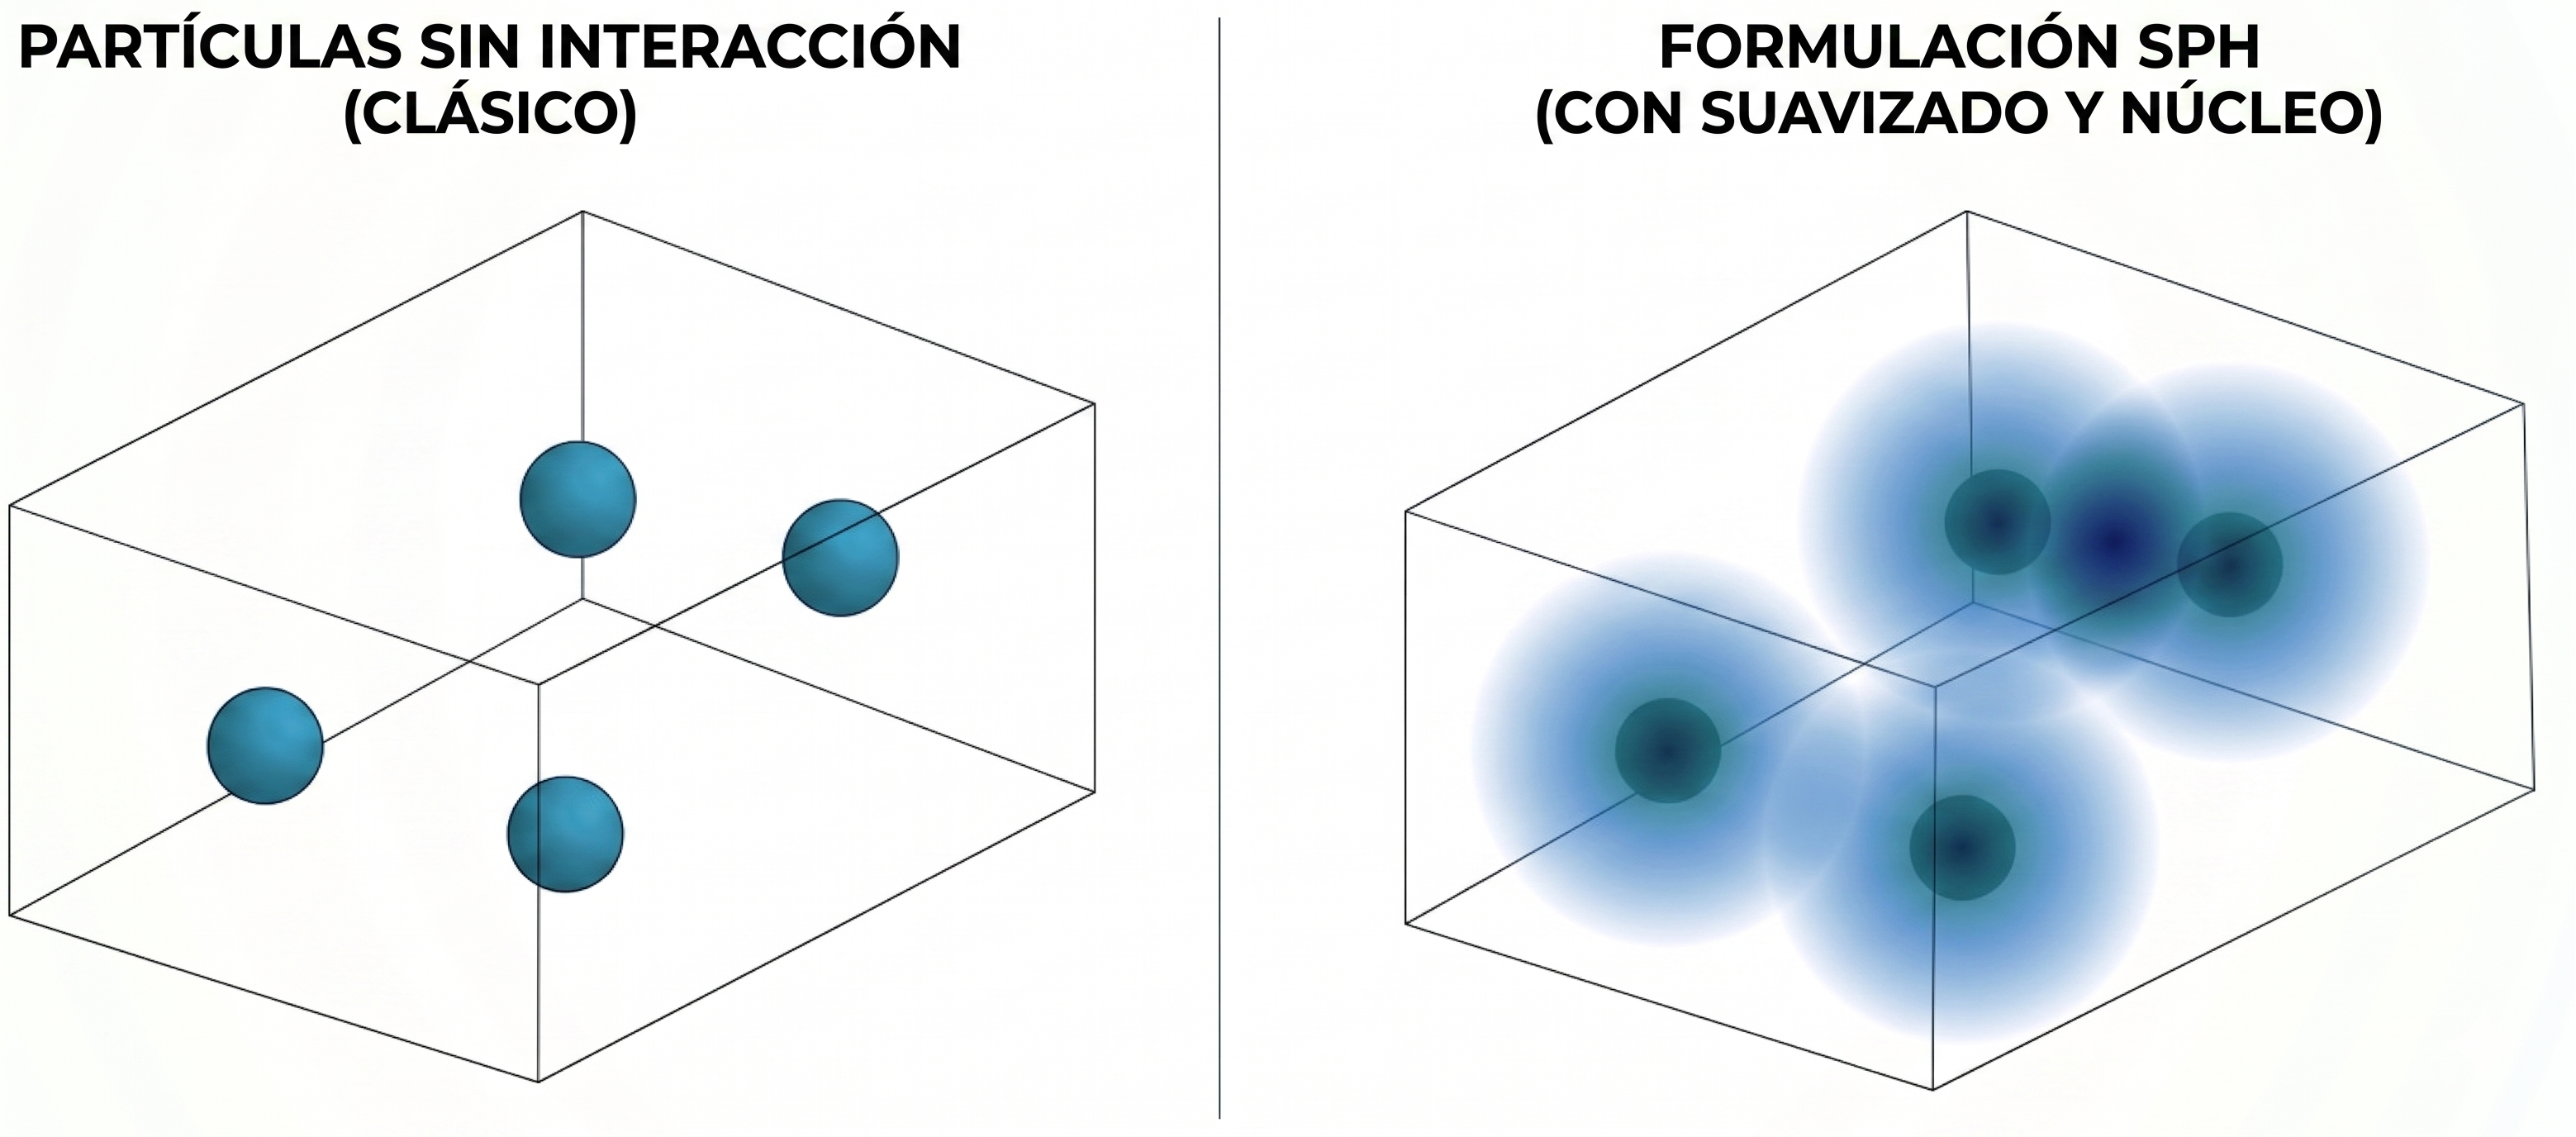
\includegraphics[width=0.8\textwidth]{chapters/cap3_macro/img/sphdifu1.png}
    \caption{Visualización conceptual de la interacción en SPH. Izquierda: partículas discretas separadas sin aparente conexión. Derecha: Difuminación de la partícula que permite solapar sus ``estelas'' o zonas de influencia, generando interacciones (definidas por el kernel) a pesar de la distancia física.}
    \label{fig:sph_difu}
\end{figure}

\subsection{Discretización de la ecuación de advección 1D}

Para comprender la ejecución computacional de este sistema discreto, tomaremos como modelo base la ecuación de advección lineal en 1D (\ref{ec: advection}). Como se definió previamente en la sección \ref{sec:adcevtion}, esta ecuación describe el transporte de una cantidad escalar a una velocidad de advección $c$, esta cantidad la llamaremos $u(x,t)$: 
\begin{equation}
    \frac{\partial u(x,t)}{\partial t} + c \frac{\partial u(x,t)}{\partial x} = 0
    \label{eq:advection_continuous}
\end{equation}

El propósito de discretizar esta ecuación es transformar la variable continua dependiente del espacio $u(x,t)$ en un conjunto finito de variables $u_j(t)$, correspondientes a cada partícula $j$ simulada en el ordenador \cite{auyeung2025}.

Aplicando la aproximación de partículas SPH al gradiente espacial de la cantidad $u$, se transita de la forma continua a una sumatoria de interacciones ponderadas por la derivada del kernel $\nabla_j W_{jk}$. Sustituyendo en la ecuación de advección diferencial y despejando para el siguiente instante temporal $t + \Delta t$ usando un esquema de Euler explícito, se obtiene la expresión completamente discretizada \cite{auyeung2025}:
\begin{equation}
    u_j(t_0 + \Delta t) = u_j(t_0) - c \Delta t \sum_{k \in \mathcal{N}_j} \left( u_k(t_0) - u_j(t_0) \right) \nabla_j W_{jk}
    \label{eq:sph_advection_discrete}
\end{equation}
donde:
\begin{itemize}
    \item $u_j(t_0)$ es el valor de la advección para la partícula de interés $j$ en el tiempo inicial $t$.
    \item $c$ es la velocidad constante de advección.
    \item $\Delta t$ es el paso de integración temporal.
    \item $\mathcal{N}_j$ representa el conjunto de partículas vecinas $k$ contenidas dentro del radio de influencia delimitado por $h$.
    \item $\nabla_j W_{jk}$ es el gradiente de la función de suavizado de la partícula $j$ con respecto a la partícula vecina $k$.
\end{itemize}

Esta formulación (ecuación \ref{eq:sph_advection_discrete}) encapsula la esencia computacional del método SPH ya que, el estado futuro de la partícula $j$ no depende de una cuadrícula estática, sino de la suma de las interacciones con sus partículas vecinas $k$, regidas por la geometría. En el caso de dos partículas fijas, ambas permanecen dentro del soporte del kernel y la ecuación~\eqref{eq:sph_advection_discrete} produce una relajación hacia la media $u=1/2$, que es precisamente el comportamiento de la referencia clásica del capítulo~\ref{cap:resultados}.



\section{Continuous-Time Quantum Walks (CTQW)}
Para llegar a una solución del advectivo planteado en la ecuación (\ref{eq:sph_advection_discrete}), en este trabajo se plantean las caminatas cuánticas. Las caminatas cuánticas en tiempo continuo (CTQW) son la contraparte cuántica de las caminatas aleatorias clásicas (procesos de Markov), formuladas originalmente para la exploración de grafos y espacios de estados discretos en computación \cite{VenegasAndraca2012}.

En un CTQW, el ``caminante'' no se mueve mediante decisiones probabilísticas paso a paso. En cambio, su amplitud de probabilidad evoluciona de manera continua a lo largo del tiempo bajo un escenario planteado por el hamiltoniano $H$ y gobernado por la ecuación de Schrödinger:
\begin{equation}
    i\hbar \frac{d}{dt} |\psi(t)\rangle = H |\psi(t)\rangle
\end{equation}

En la teoría de grafos cuánticos, el hamiltoniano $H$ que rige esta evolución se define directamente a través de la matriz de adyacencia $A$ del grafo (o su Laplaciano $L$). De este modo, la evolución unitaria temporal del estado cuántico está dada por el operador $U(t) = e^{-iHt}$. Esta característica hace a los CTQW una herramienta interesante para la simulación física, ya que, la dinámica del sistema modela fielmente las tasas de transición directa entre los nodos \cite{VenegasAndraca2012}.

% chapters/cap4_metod/cap4.tex

\chapter{Metodología}
\label{cap:metodologia}

En este capítulo se describe de manera detallada la metodología aplicada para la resolución de la ecuación de advección unidimensional para dos partículas SPH. A partir de la base teórica establecida, se detalla el modelado del problema y la transición hacia las caminatas cuánticas de tiempo continuo y las consideraciones físicas necesarias para su implementación.

\section{Análisis del trabajo previo}

Es fundamental resaltar el trabajo previo realizado en \cite{auyeung2024, auyeung2025}, el cual establece las bases teóricas de \emph{Quantum SPH} (QSPH). En su investigación, se realiza de forma detallada la formulación matemática que traduce la dinámica clásica de partículas SPH \eqref{eq:sph_advection_discrete}, a un formalismo válido dentro de la mecánica cuántica. Siguiendo este trabajo, la formulación a la que se llega para ver el paso del tiempo de la cantidad advectada $u$ en la partícula $j$ está dada por:

\begin{equation}
    u_j(t_0 + \Delta t) = u_j(t_0) - c \Delta t \, v N |\mathbf{a}| \Re(\langle a | \nabla_j W_{jk} \rangle)
    \label{eq:auyeung}
\end{equation}

Esta ecuación demuestra que es posible alcanzar estados válidos que representan la dinámica del fluido, por medio de QSPH, en un computador cuántico. Partiendo de esta base, y asumiendo por simplicidad una separación espacial uniforme entre las partículas ($\Delta x_k = \Delta x$) para un paso de tiempo constante $\Delta t$, en \cite{auyeung2025} reescriben la ecuación de advección SPH de la siguiente manera:

\begin{equation}
    u_j(t_0+1) = u_j(t_0) - c N \Delta x \sum_{k \neq j} V_{jk} + c N \Delta x \sum_{k \neq j} u_k(t_0) V_{jk}
    \label{eq:auyeung_14}
\end{equation}

donde $V_{jk} = \nabla_j W_{jk}/(vN) + ib_{jk} $ y $v = \max|\nabla_j W_{jk}|$. De esta forma se encapsula la evaluación del kernel de suavizado junto con los términos de normalización imaginarios necesarios para garantizar la unitariedad en el computador cuántico. Para adaptar esta expresión al formalismo de las caminatas cuánticas continuas (CTQW), los autores definen las amplitudes de probabilidad, equivalentes a los coeficientes de evolución temporal. La amplitud de autointeracción para la partícula $j$ se define como:

\begin{equation}
    \alpha_{jj} = 1 + c N \Delta x \Re(\sum_{k \neq j} V_{jk})
    \label{eq:auyeung_15}
\end{equation}

mientras que la amplitud de interacción que gobierna el flujo desde las partículas vecinas $k$ hacia $j$ está dada por:

\begin{equation}
  \alpha_{jk} = -c N \Delta x \Re(V_{jk})
    \label{eq:auyeung_16}
\end{equation}

Sustituyendo estas amplitudes en la ecuación \eqref{eq:auyeung_14}, se llega a la forma compacta de la actualización temporal que dicta cómo evoluciona la cantidad advectada $u_j$:

\begin{equation}
    u_j(t_0+1) = \alpha_{jj} u_j(t_0) + \sum_{k} \alpha_{kj} u_k(t_0)
    \label{eq:auyeung_17}
\end{equation}

Esta formulación define valores de una matriz de evolución temporal a través de la formación de los coeficientes $\alpha_{jj}$ \eqref{eq:auyeung_15}, $\alpha_{jk}$ \eqref{eq:auyeung_16}, en los cuales lleva consigo toda la información del escenario y la interacción con cada partícula.

No obstante, la formulación alcanzada en dichos trabajos no representa un SPH puro en su concepción lagrangiana. Debido a la formulación QSPH \eqref{eq:auyeung}, las partículas no se encuentran libres; en su lugar, se asume un $\Delta x$ constante que no varía con el tiempo ni con la interacción. Las partículas permanecen fijas en un espacio definido. Aunque los autores reconocen esta limitación, este paradigma nos motiva a replantear el problema desde la naturaleza de un CTQW. Ese anclaje de posiciones es también el de este TFM y explica que el dímero tenga una relajación en lugar de advectar un perfil.


\section{Analogía con CTQW}
\label{subsec: analogía}

En la exploración de grafos mediante CTQW, los nodos permanecen fijos en el espacio y no dependen estrictamente de los nodos circundantes para definir su posición. Sin embargo, la información que fluye a través del grafo, su amplitud de probabilidad, sí depende de la topología local (sus vecinos y el escenario general). Esta dinámica exhibe un paralelismo profundo con una malla euleriana o un escenario SPH predefinido, donde dejamos que la ``información'' (el fluido) se propague a través de los nodos estáticos.

Para ver de forma matemática esta relación, definimos un grafo $G$ estructurado por una matriz de adyacencia $M_{ab}$ de tamaño $n \times n$, donde $n$ es el número de vértices (que se puede asemejar a partículas).

\begin{equation}
    M_{ab} = 
    \begin{cases} 
        -\gamma, & a \neq b, \ (a,b) \in G \\
        0, & a \neq b, \ (a,b) \notin G \\
        k\gamma, & a = b
    \end{cases}
    \label{eq:matriz_Mab}
\end{equation}

Los coeficientes de $M_{ab}$ dictan el peso de las conexiones (edges) entre un nodo $a$ y un nodo $b$. La variación de la probabilidad $P_a(t)$ de encontrar al caminante en el nodo $a$ con respecto a sus vecinos se describe típicamente como:

\begin{equation}
    \frac{d P_a(t)}{dt} = - \sum_b M_{ab} P_b(t)
    \label{eq:prob_variation}
\end{equation}

Esta expresión ya muestra una forma análoga a la discretización SPH y para poder ver una semejanza hay que ver la dinámica de un sistema cerrado que, en mecánica cuántica, esto se rige por la ecuación de Schrödinger:

\begin{equation}
    i \frac{d}{dt} \langle a | \psi(t) \rangle = \sum_b \langle a | H | b \rangle \langle b | \psi(t) \rangle
    \label{eq:schrodinger}
\end{equation}

En el cual podemos encontrar una relación importante para el desarrollo de este trabajo, $\hat{H} = \langle a | H | b \rangle \langle b \rangle = M_{ab}$, el hamiltoniano $H$ se diseña directamente a partir de la matriz de adyacencia ($H \propto M_{ab}$). Esto nos define el operador de evolución unitaria en un CTQW como: $\hat{U} = e^{-i\hat{H}t}$. \cite{VenegasAndraca2012}. 

La analogía es directa, tanto la ecuación \eqref{eq:auyeung_17} y la \eqref{eq:schrodinger} definen un escenario donde la variación del estado local (ya sea amplitud de probabilidad $\langle a | \psi(t) \rangle$ o la cantidad advectada $u_j$) depende de la influencia directa de sus vecinos mediante coeficientes topológicos. De modo que en este trabajo se intenta implementar un CTQW para poder ver el comportamiento de la cantidad advectada en el tiempo. 

\section{Construcción de matriz hermítica para el Hamiltoniano}
\label{sec:Contruccion_J}

El primer aspecto a considerar en la transición hacia un modelo cuántico continuo es que la matriz de evolución de tiempo discreto $\alpha$, formada por \eqref{eq:auyeung_15} y \eqref{eq:auyeung_16} no es compatible de forma directa con la mecánica de un Hamiltoniano de \textit{Continuous-Time Quantum Walk} (CTQW), fundamentalmente porque dicha matriz no es hermítica. En la matriz original, los términos de la diagonal principal $\alpha_{jj}$ representan la probabilidad de permanencia en el mismo nodo; es decir, la probabilidad de que la información no salte hacia otra partícula. Esta formulación es sumamente útil en los \textit{Discrete-Time Quantum Walks} (DTQW), ya que en ese paradigma se utiliza un operador moneda (\textit{coin operator}) para gobernar explícitamente la decisión de saltar o quedarse. 

Sin embargo, las mecánicas del CTQW operan bajo un principio topológico distinto. En este modelo ya no disponemos de un operador moneda que dicte el comportamiento paso a paso. En su lugar, el sistema define un ``escenario'' construido enteramente a partir del acoplo entre partículas. Dejamos que el estado del sistema cuántico evolucione de forma natural y continua dentro de este escenario, de modo que las transiciones ocurren en función de la fuerza de las interacciones dictadas por el grafo.

Para construir un Hamiltoniano válido que represente este escenario, necesitamos definir una matriz $J$ que sea hermítica. Partiendo de la matriz $\alpha$, procedemos a anular los valores de permanencia en el nodo estableciendo $\alpha_{jj} = 0$. Esta elección cambia el generador respecto a \cite{auyeung2024}, ya que no se implementa la autointeracción discreta como término diagonal unitario. La relajación de la ecuación (\eqref{eq:sph_advection_discrete}), no se busca en $\alpha_{jj}$, sino en el mapa abierto del capítulo~\ref{cap:implementacion_circuito}. Esta simplificación constituye la reinterpretación hermítica mínima del subespacio de dos partículas para el CTQW. De este modo, aislamos exclusivamente los valores de acoplo cruzado, obteniendo la siguiente matriz:

\begin{equation}
J = 
\begin{pmatrix}
0 & \alpha_{01} \\
\alpha_{10} & 0
\end{pmatrix}
\end{equation}

Esta estructura matricial hermítica será la base para la construcción del circuito cuántico. A continuación, es preciso analizar la composición interna del término $\alpha$. Para el presente trabajo se ha escogido una función de kernel triangular, cuya representación analítica en función del radio de suavizado $h$ y la distancia relativa $r$ viene dada por:

\begin{equation}
W(r,h) = \frac{1}{h} - \frac{|r|}{h^2} \quad \text{para} \quad |r| < h
\end{equation}

La derivada espacial de este kernel, la cual se usa para el cálculo de las interacciones SPH, resulta en:

\begin{equation}
\frac{dW(r,h)}{dr} = -\frac{\text{sgn}(r)}{h^2} \quad \text{para} \quad |r| < h
\end{equation}

Para comprender la dinámica de salto, evaluemos el cálculo del coeficiente $\alpha_{01}$. Partiendo de la formulación SPH para una sola partícula vecina, el término se define como $\alpha_{01} = -c \cdot v \cdot N \cdot \Delta x \cdot V_{01}$. Aquí, $V_{01}$ se calcula como $V_{01} = \frac{\nabla_0 W_{01}}{v N}$, donde $v = \max|\nabla_j W_{jk}|$. 

Al emplear el kernel triangular, y considerando el sistema de 2 partículas, el valor máximo del gradiente es $v = \frac{1}{h^2}$. Puesto que el gradiente se evalúa desde la partícula 0 hacia la partícula 1, tenemos que $\nabla_0 W_{01} = -\frac{1}{h^2}$. Sustituyendo estos valores, observamos que $V_{01}$ se reduce a $-1/N$. Al introducir este resultado en la ecuación principal, los signos se cancelan, dejando:

\begin{equation}
\alpha_{01} = c \cdot v \cdot |\Delta x|
\label{eq: alfa}
\end{equation}

Aplicando el mismo desarrollo por simetría, obtenemos un resultado idéntico para $\alpha_{10}$.

\begin{figure}[htbp]
    \centering
    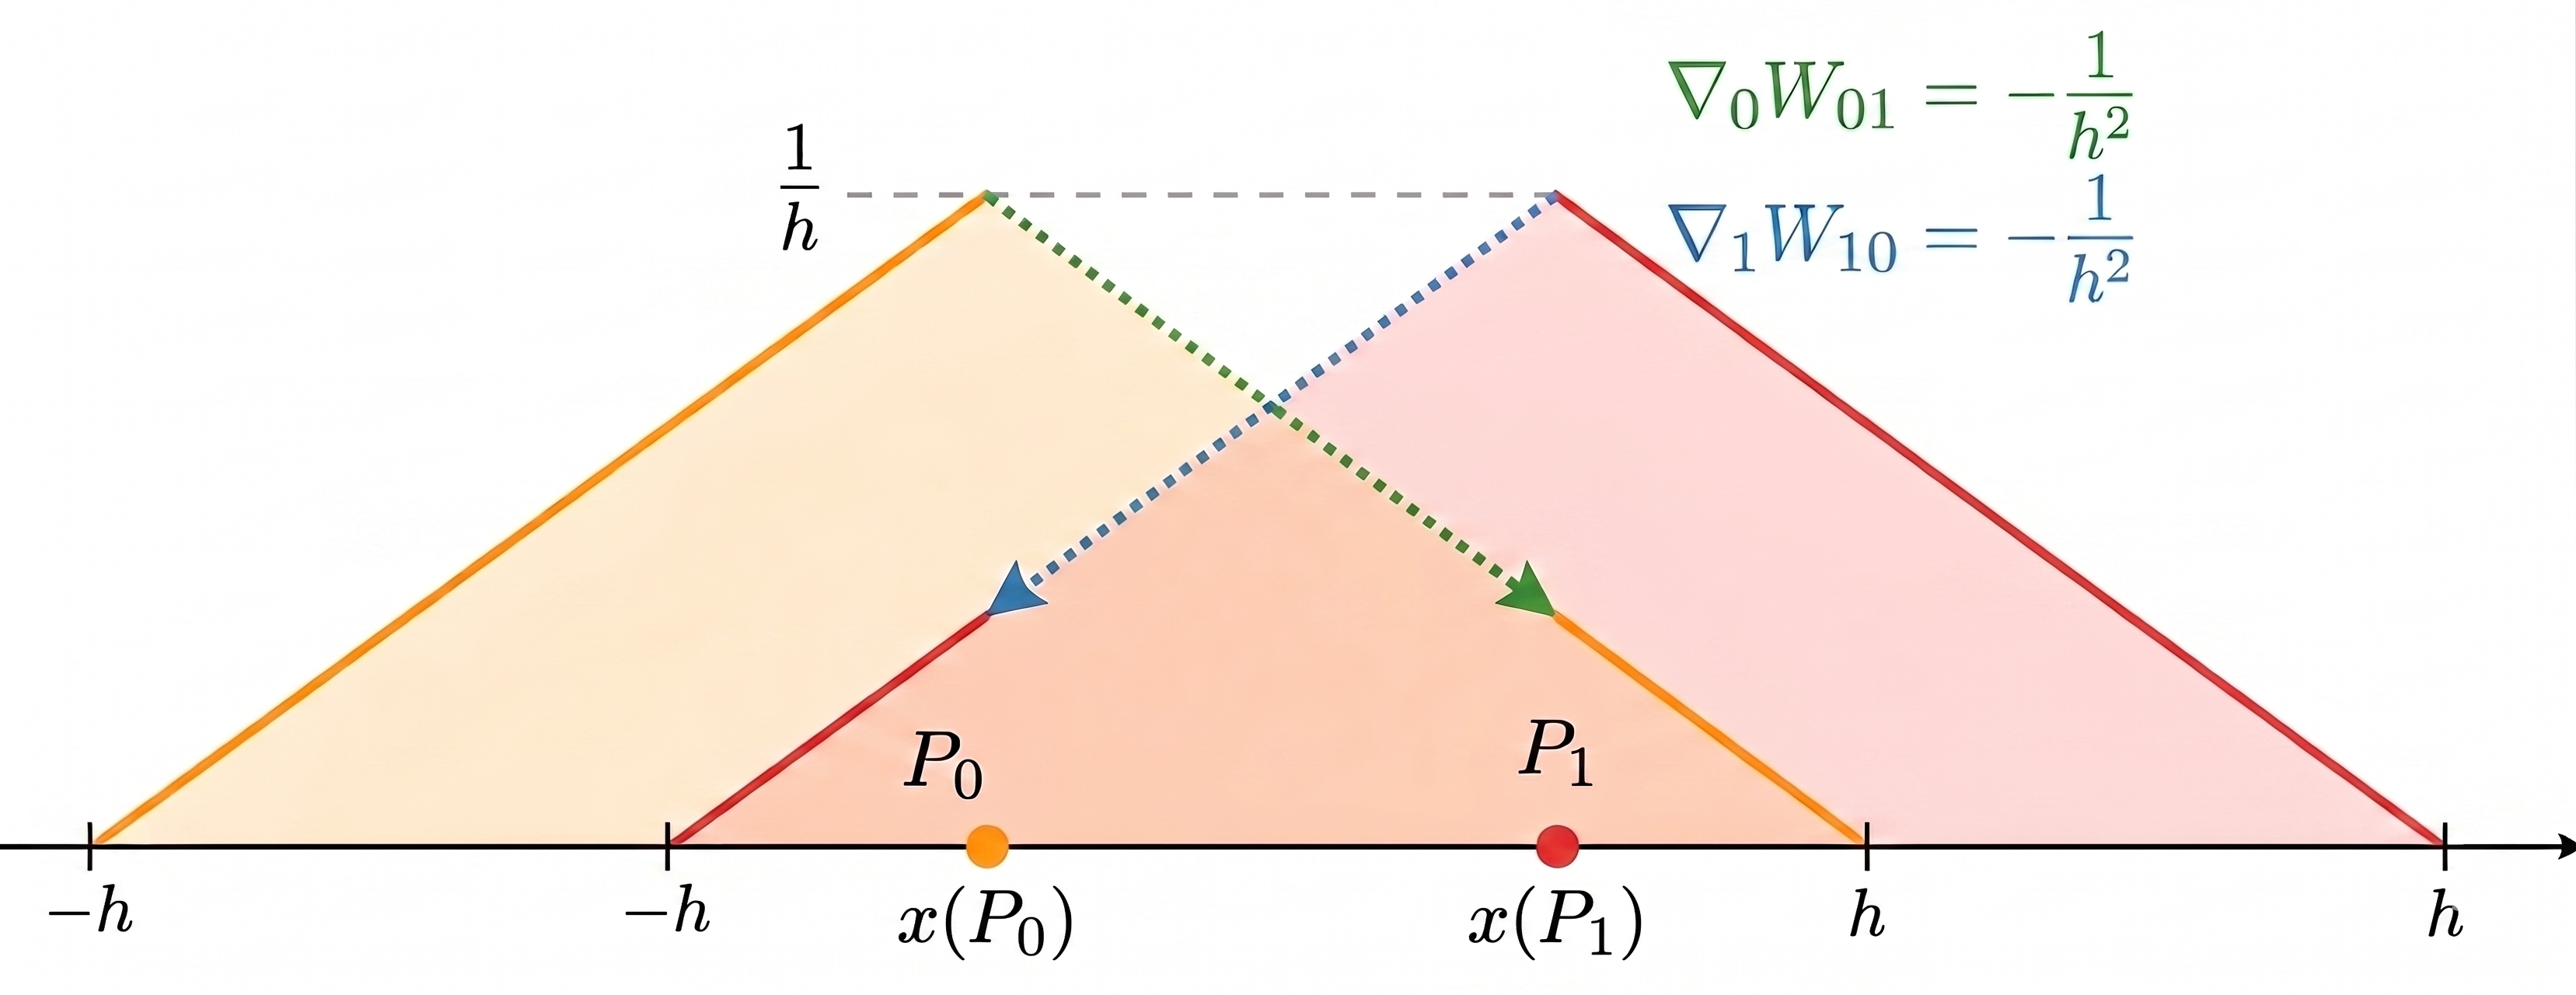
\includegraphics[width=0.9\textwidth]{chapters/cap4_metod/img/kernel_esquema.png}
    \caption{Esquema geométrico del kernel triangular y la dirección de interacción entre partículas.}
    \label{fig:kernel_esquema}
\end{figure}

Para visualizar este comportamiento de forma más gráfica, podemos remitirnos a la figura \ref{fig:kernel_esquema}. El hecho de que el valor final de $\alpha$ sea positivo obedece a una convención física fundamental, la cual implica que siempre evaluamos la derivada del kernel desde el punto de vista de la partícula $j$ hacia la partícula $k$, y nunca a la inversa. Al incorporar el operador $\nabla_j$, garantizamos que la derivada direccional sea negativa, lo que a su vez hace que la sumatoria $V_{jk}$ sea consistentemente negativa y, al multiplicarse por el signo de la ecuación, el término final $\alpha$ resulte positivo. 

Físicamente, este formalismo tiene total sentido dentro de la hidrodinámica de partículas suavizadas (SPH). Si una partícula penetra en el radio de interacción $h$ de su vecina, la geometría del kernel genera una fuerza de repulsión que cada vez debe ser más fuerte mientras más se junten las partículas, por eso un fluido se comprime hasta un límite. Si por el contrario el término $\alpha$ fuera negativo, estaríamos ante una fuerza de atracción, lo cual es inviable e inestable en este contexto. Todas las propiedades del fluido emergen de esta derivada del kernel, la cual presenta un pico de interacción máxima justo en la posición de la partícula. Son estas distintas geometrías del kernel las que, en última instancia, dictarán las propiedades macroscópicas como la viscosidad.

Finalmente, incorporando estos resultados, la matriz hermítica completa $J$ que define nuestro escenario interactivo queda conformada de la siguiente manera: 

\begin{equation}
J = 
\begin{pmatrix}
0 & c \cdot v \cdot \Delta x \\
c \cdot v \cdot \Delta x & 0
\end{pmatrix}
\label{mat: J}
\end{equation}

Con la obtención de esta matriz hermítica $J$, hemos consolidado el hamiltoniano del sistema. En el siguiente capítulo, se propone la construcción de esta matriz directamente a un circuito para computadores cuánticos universales empleando el método de \textit{Matching Decomposition}.

\section{Codificación del estado físico}
\label{sec:codificacion_estado}

Una vez definido el hamiltoniano $J$, que actúa como el escenario donde están embebidas todas las relaciones espaciales y topológicas dictadas por el kernel SPH, es necesario la definición formal entre la variable de interés del fluido (la cantidad advectada $u$) y el estado del sistema cuántico. 

Para un sistema de $N=2$ partículas, el espacio de estados puede ser representado íntegramente utilizando un único qubit, el cual define un espacio de Hilbert bidimensional $\mathcal{H} \cong \mathbb{C}^2$. En este esquema, los estados ortonormales de la base computacional identifican a las partículas mismas como entidades (o contenedores) de la propiedad física. Así, definimos:
\begin{itemize}
    \item $|0\rangle$: Representa a la partícula 0 como portadora de la cantidad advectada.
    \item $|1\rangle$: Representa a la partícula 1 como portadora de la cantidad advectada.
\end{itemize}

Para introducir la magnitud de la cantidad advectada en el computador cuántico, se recurre a la técnica de codificación por amplitud, (\textit{Amplitude Encoding}). Siguiendo la analogía descrita en la sección \ref{subsec: analogía}, el valor escalar de la cantidad advectada $u_j(t)$ en la partícula $j$ se codifica directamente como la amplitud de probabilidad del estado base correspondiente. Por lo tanto, el estado global del fluido en cualquier instante $t$ se describe mediante el vector de estado:

\begin{equation}
    |\psi(t)\rangle = u_0(t)|0\rangle + u_1(t)|1\rangle
    \label{eq:estado_cuantico}
\end{equation}

La preparación es, por tanto, un \textit{amplitude encoding}. La lectura, en cambio, se hace en la base computacional, dando como resultado que los \textit{shots} estiman las poblaciones $P_j = \rho_{jj}$. En este trabajo se identifica el escalar SPH con esas poblaciones, $u_j(t) \leftrightarrow P_j(t)$, que es la cantidad que se compara con la ecuación~\eqref{eq:sph_advection_discrete} en el capítulo~\ref{cap:resultados}.

Bajo esta formulación, el escenario espacial (la distancia entre las partículas y la fuerza de su interacción) queda dictado por el hamiltoniano. El vector de estado $|\psi(t)\rangle$ se limita a describir cómo fluye y se distribuye la cantidad advectada entre las partículas.

La normalización $\langle\psi|\psi\rangle = 1$ (o $\mathrm{Tr}\,\rho = 1$ en el caso abierto) es un postulado cuántico; no es el mismo enunciado que la conservación de masa del dímero clásico $u_0 + u_1$. En este experimento el escalar SPH se identifica con la población, $u_j^{\text{(leída)}} := P_j = \rho_{jj}$, y esa es la curva que se compara con \eqref{eq:sph_advection_discrete} en el capítulo~\ref{cap:resultados}. No se aplica $\sqrt{P_j}$ ni tomografía de amplitudes. En el circuito abierto el estado es, en general, mixto: no hay una única amplitud compleja que recuperar. El rango ficticio $u \in [0,1]$ hace legítima esa identificación en $N=2$; para magnitudes físicas con otra escala haría falta un factor clásico de normalización \textbf{antes} del \textit{encoding}, y la lectura seguiría siendo $P_j$, no $\sqrt{P_j}$.

Para el caso de estudio de este trabajo, establecemos como condición inicial que el 100\% de la cantidad advectada se encuentra concentrada en la partícula 0 en el instante $t=0$. En términos del vector de estado, esta condición se expresa como:

\begin{equation}
    |\psi(0)\rangle = 1|0\rangle + 0|1\rangle = |0\rangle
    \label{eq:condicion_inicial}
\end{equation}

Con el estado inicial definido y el hamiltoniano $J$ construido (\ref{mat: J}), la evolución analítica del sistema se rige por la aplicación del operador de evolución temporal unitaria $\hat{U}(t) = e^{-i J t}$. Las puertas universales para la ejecución de este operador $\hat{U}$ y su análisis se realiza en el siguiente capítulo.



% chapters/cap5_circuito/cap5.tex
\chapter{Diseño e Implementación del Circuito Cuántico}
\label{cap:implementacion_circuito}

En el capítulo anterior se estableció la formulación matemática para la discretización espacial de la hidrodinámica de partículas suavizadas (SPH) en un formalismo cuántico. Específicamente, se definió la construcción de una matriz hermítica, la cual actúa directamente como el hamiltoniano $H$ del sistema continuo (Continuous-Time Quantum Walk, CTQW). En el presente capítulo, se describe el proceso seguido para traducir el operador de evolución temporal a un circuito de puertas cuánticas universales.

\section{Descomposición de emparejamiento (Matching Decomposition)}
\label{sec:matching_decomposition}

La simulación de la dinámica de un sistema cuántico cerrado dictado por un hamiltoniano $H$ requiere la implementación del operador de evolución temporal $U(t) = e^{-iHt}$. En el contexto de este trabajo, $H$ corresponde a la matriz hermítica mínima a partir de adyacencia del grafo ponderado definido por las interacciones de las partículas SPH. Tradicionalmente, la simulación de estos operadores en hardware cuántico universal se realiza mediante la Descomposición de Pauli (\emph{Pauli Decomposition}). Este método estándar proyecta el hamiltoniano en una base de cadenas de operadores de Pauli $P_j \in \{I, X, Y, Z\}^{\otimes n}$, de forma que $H = \sum_{j} c_j P_j$. Sin embargo, este enfoque tiene una limitación de escalabilidad, ya que, para un grafo de $N = 2^n$ nodos, la descomposición puede generar hasta $\mathcal{O}(N^2)$ términos no locales, lo que se traduce en circuitos con una profundidad excesiva y una alta densidad de puertas $CNOT$, haciéndolos inviables en la era $NISQ$ (\emph{Noisy Intermediate-Scale Quantum}).

Para intentar abordar esta limitación y lograr un circuito viable, en este trabajo se emplea la descomposición de emparejamiento (\textit{Matching Decomposition}), propuesta en \cite{matching2026}. Este método aprovecha la topología inherente del grafo de interacciones para descomponer el hamiltoniano sin transitar por el espacio de Pauli, operando directamente sobre las aristas del grafo.

Sea $G = (V, E)$ el grafo cuyas aristas están ponderadas por el kernel SPH. Un emparejamiento o \textit{matching} $M$ se define como un subconjunto de aristas $E$ tal que ningún par de aristas en $M$ comparte un vértice común. El teorema de Vizing garantiza que las aristas de cualquier grafo con grado máximo $\Delta$ pueden ser particionadas (coloreadas) en a lo sumo $\Delta + 1$ emparejamientos disjuntos. Así, el hamiltoniano total se puede expresar como la suma de hamiltonianos parciales, cada uno correspondiente a un emparejamiento:
\begin{equation}
    H = \sum_{k=1}^{\chi} H_{M_k}
\end{equation}
donde $\chi \leq \Delta + 1$ es el índice cromático del grafo y $H_{M_k}$ contiene únicamente interacciones entre pares de vértices aislados temporalmente del resto de la red, \cite{vizing1964estimate}.

La ventaja crítica de esta formulación radica en la conmutatividad local. Dado que las aristas dentro de un mismo emparejamiento $M_k$ no comparten vértices, los operadores de evolución correspondientes a cada arista dentro de $M_k$ conmutan estrictamente entre sí. Por lo tanto, el operador de evolución temporal para el sub-hamiltoniano $H_{M_k}$ puede aplicarse de manera exacta y en paralelo:
\begin{equation}
    e^{-i H_{M_k} t} = \prod_{(u,v) \in M_k} e^{-i w_{u,v} \sigma_{x}^{(u,v)} t}
\end{equation}
donde $w_{u,v}$ representa el peso del kernel SPH entre las partículas $u$ y $v$. La transición a la evolución global del sistema se aproxima utilizando la fórmula de Trotter-Suzuki de primer orden (o superior):
\begin{equation}
    e^{-i H t} \approx \left( \prod_{k=1}^{\chi} e^{-i H_{M_k} \frac{t}{r}} \right)^r
\end{equation}
donde $r$ es el número de pasos de Trotter, \cite{suzuki1976generalized}. 

A nivel de circuito, cada interacción bidireccional entre nodos $(u,v)$ en la base computacional se implementa utilizando rotaciones controladas ($CR_x$) enmarcadas por puertas $CNOT$ para aislar el subespacio de los dos estados involucrados. Al implementar directamente la conectividad geométrica del fluido SPH, en grafos generales \textit{Matching Decomposition} puede reducir el número de operaciones de entrelazamiento. Según lo demostrado en \cite{matching2026}, este enfoque logra reducir la cantidad de puertas $CX$ hasta en un $43\%$ y acortar la profundidad del circuito en un $54\%$ frente a métodos convencionales, lo cual es interesante en este trabajo para mantener la coherencia del estado cuántico durante la simulación de la advección. Esas reducciones corresponden a los grafos estudiados por dichos autores. En el dímero de este trabajo el \textit{matching} es trivial y cada paso de Trotter se reduce a una rotación $R_x$ (figura~\ref{fig:circuito_1}); no se reporta aquí una ganancia de $CX$ propia.

\section{Primera implementación}
\label{sec:primera_implementacion}

Como primera aproximación al problema, se empleó directamente la matriz de adyacencia definida en la ecuación \ref{mat: J}, aplicando el método de \textit{Matching Decomposition} descrito en la sección \ref{sec:matching_decomposition}. Para esta simulación inicial, se adoptaron los parámetros físicos propuestos por Au-Yeung \textit{et al.} \cite{auyeung2025}: $h = 1.2$, $\Delta x = 0.5$, $c = 10^{-0.5}$ y $v = 1.0 / h^2$. La velocidad de advección $c$ fue seleccionada específicamente basándose en los experimentos de la literatura \cite{auyeung2025}, ya que promueve una mayor interacción de la cantidad advectada entre las partículas.

Al calcular los coeficientes $\alpha$ de la ecuación \ref{eq: alfa} con estos parámetros, se obtiene la siguiente matriz hermitiana $J$ para un sistema de dos partículas:

\begin{equation}
    J = 
    \begin{pmatrix}
    0 & 0.1098 \\
    0.1098 & 0
    \end{pmatrix}
    \label{mat: J_classical}
\end{equation}

Esta matriz $J$ actúa como el hamiltoniano del sistema. Para su traducción computacional, se desarrolló un algoritmo en Python utilizando la librería Qiskit, el cual implementa el pseudocódigo propuesto en \cite{matching2026}. Este programa toma la matriz y devuelve un circuito cuántico optimizado. 

Para gestionar la evolución temporal, es necesario discretizar el tiempo total de simulación mediante la fórmula de Trotter-Suzuki. Se definió un tiempo final objetivo de $t_{final} = 30$, descompuesto en $r = 100$ pasos de Trotter. Esto establece un paso de tiempo físico $\Delta t = 0.3$. De este modo, cada bloque de Trotter en el circuito representa la evolución del fluido durante un instante $\Delta t$. En la figura \ref{fig:circuito_1} se ilustra el circuito resultante para un único bloque de Trotter, el cual, gracias a la simplicidad del caso de dos partículas y la eficiencia del \textit{Matching Decomposition}, se reduce a una única puerta de rotación $R_x(0.65881)$ por cada $\Delta t$, como corresponde a un único emparejamiento en $N=2$. Para alcanzar el tiempo final $t_{final}$, este bloque debe aplicarse 100 veces.

\begin{figure}[htbp]
    \centering
    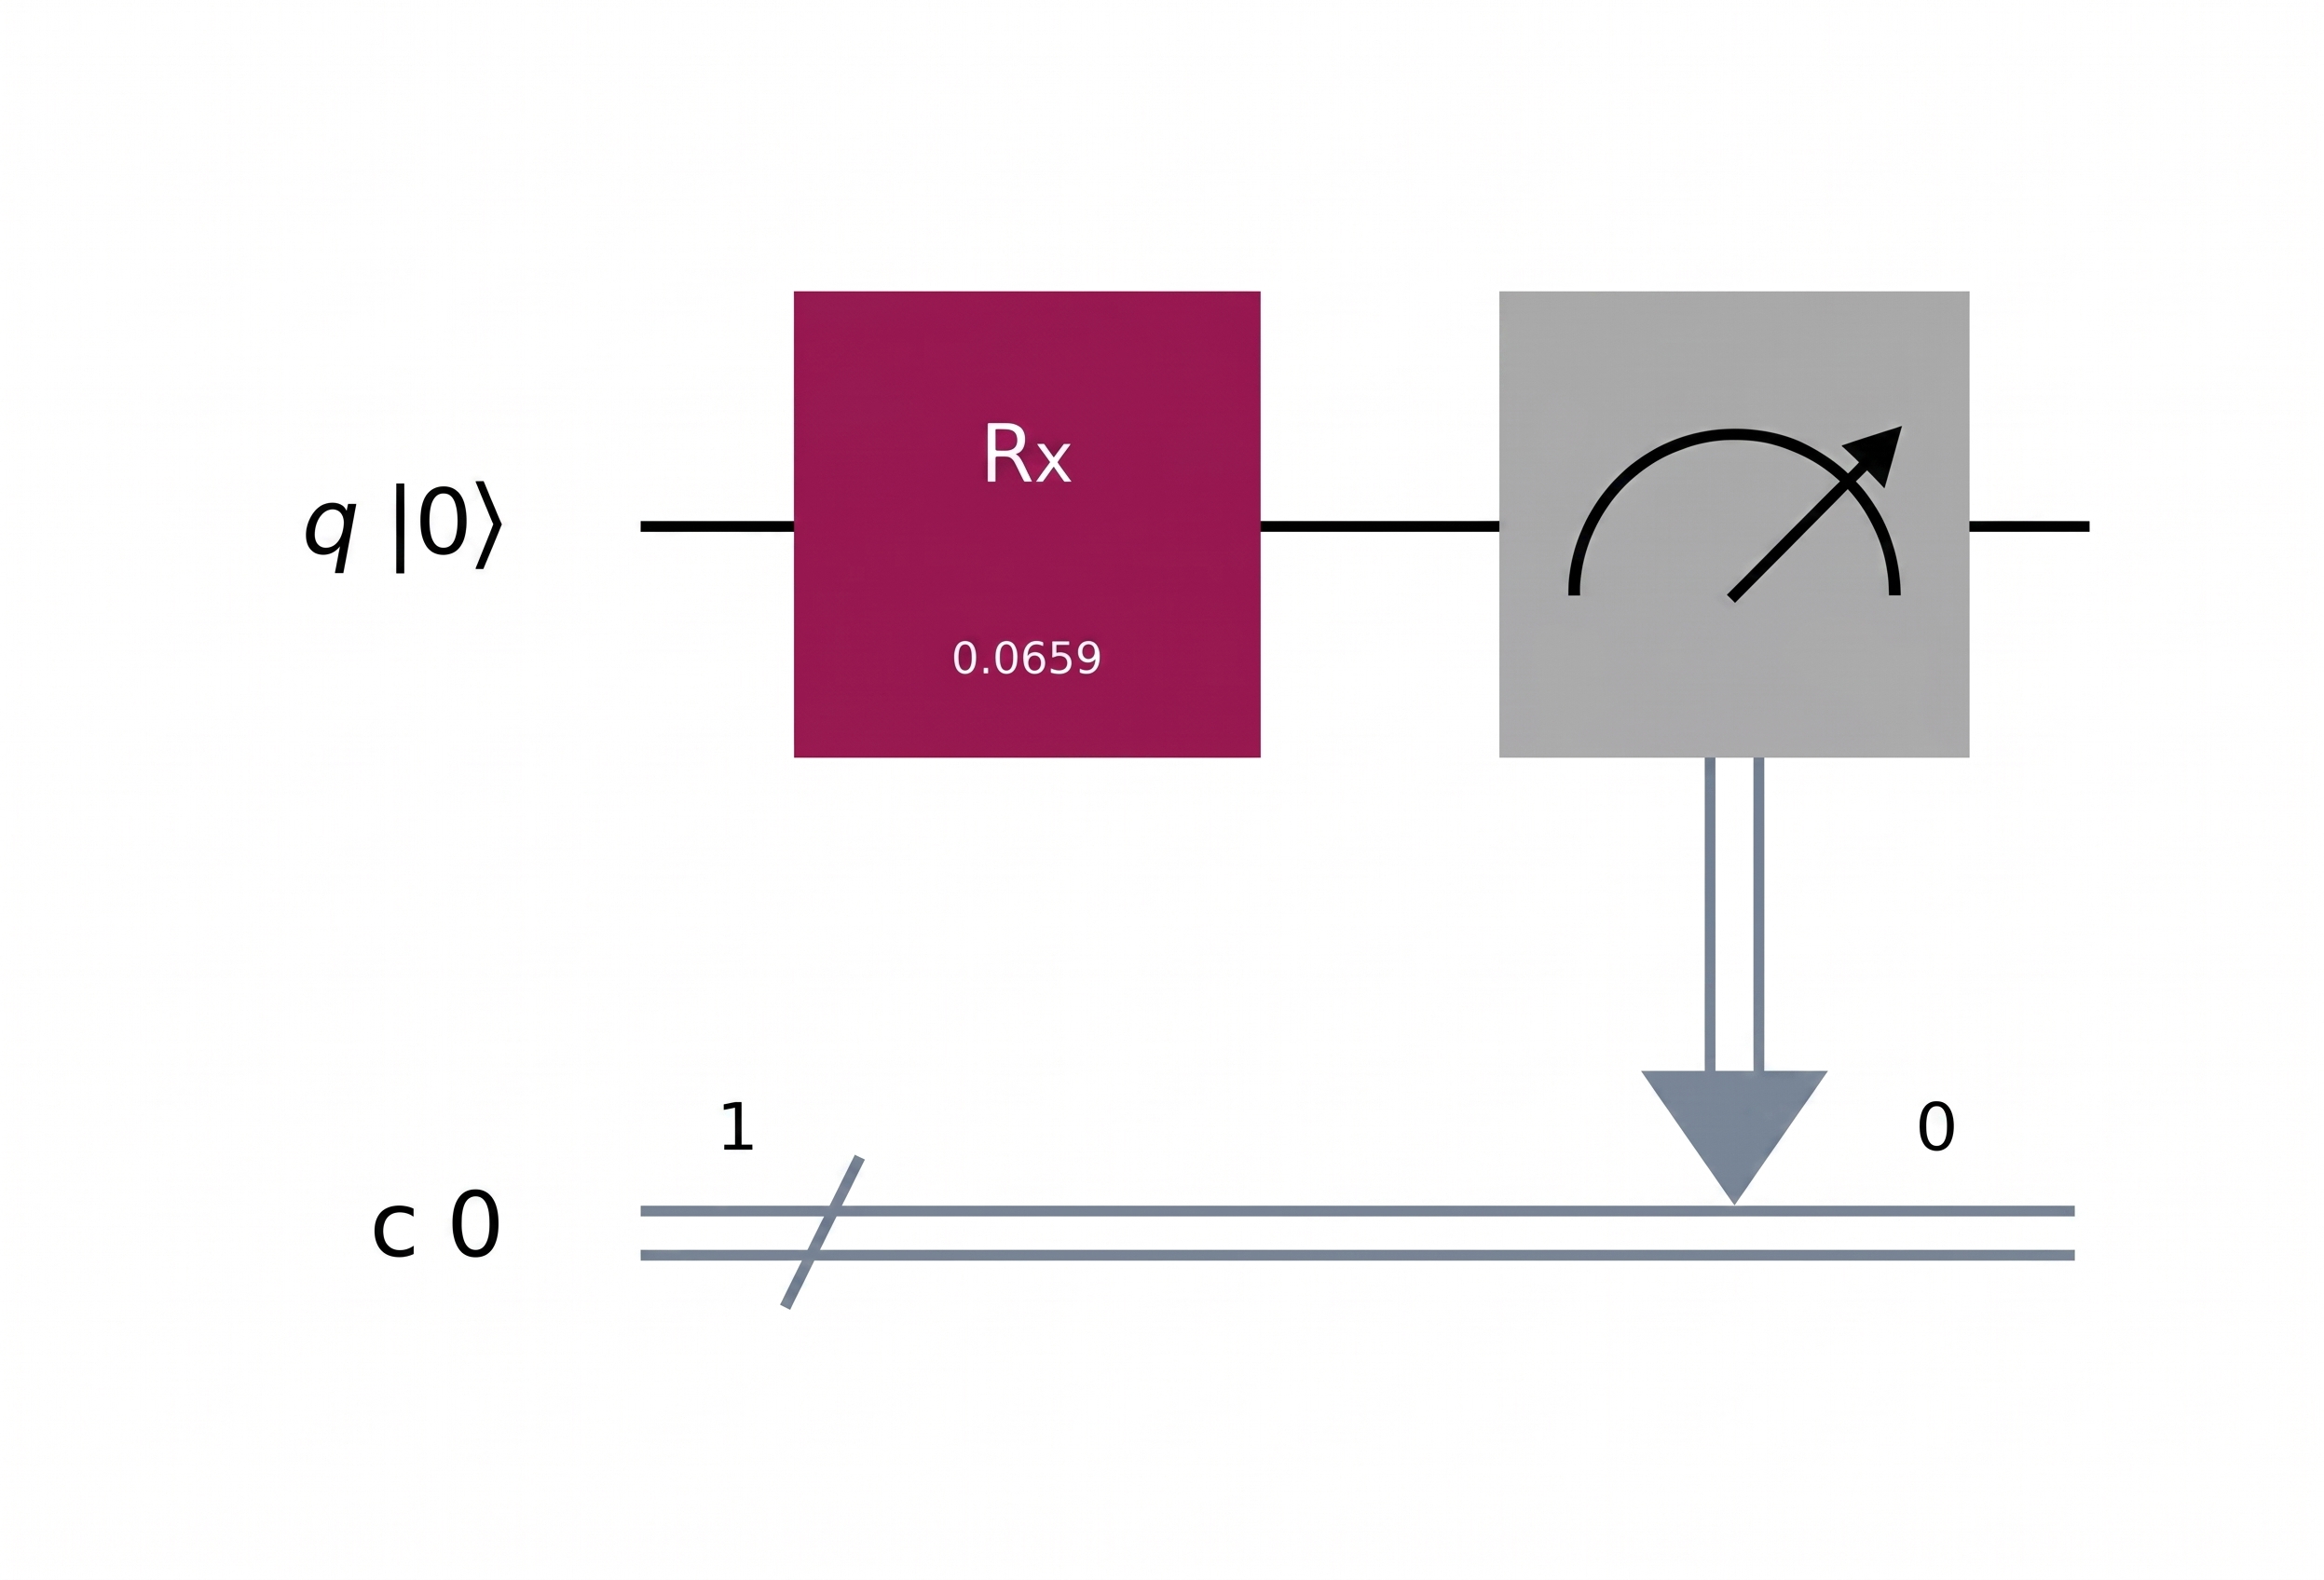
\includegraphics[width=0.6\textwidth]{chapters/cap5_circuito/img/circuito_1.png}
    \caption{Implementación de un único bloque de Trotter correspondiente a un paso de tiempo $\Delta t = 0.3$. La interacción del kernel SPH se traduce en una rotación $R_x$ sobre los qubits del sistema.}
    \label{fig:circuito_1}
\end{figure}

Para evaluar la dinámica del circuito, se realizaron simulaciones con 4000 \textit{shots} (mediciones) por cada ejecución. Con el fin de tener una resolución legible en la dinámica temporal, la gráfica se construyó muestreando únicamente 30 puntos distribuidos uniformemente a lo largo de los 100 pasos de Trotter. Los resultados se muestran en la figura \ref{fig:resultado_1}, donde se representan las poblaciones $P_j$ del qubit del sistema.

\begin{figure}[htbp]
    \centering
    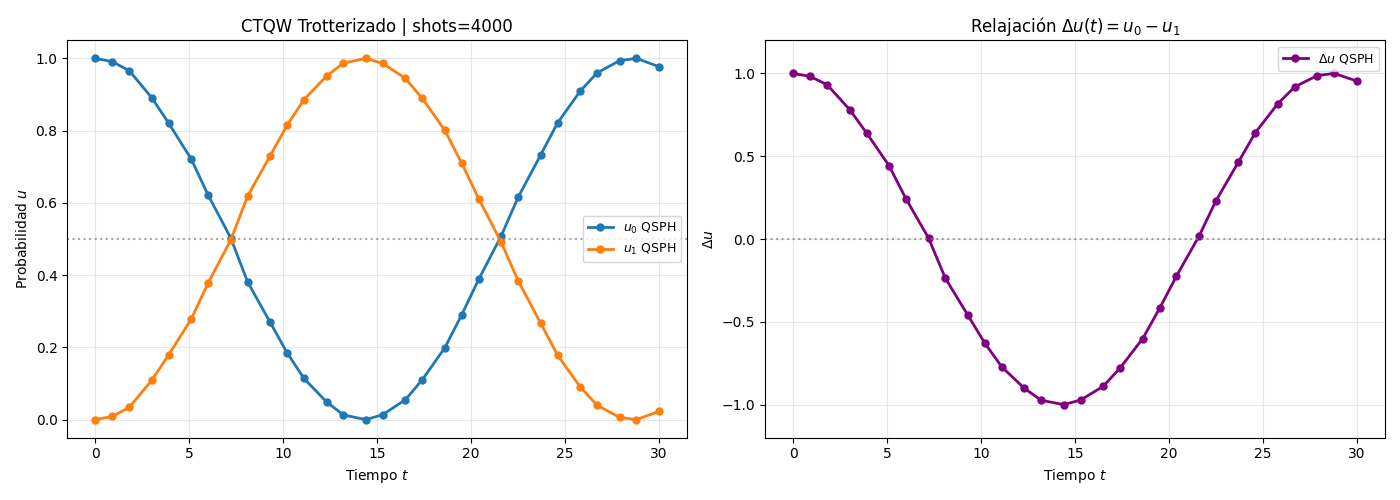
\includegraphics[width=1\textwidth]{chapters/cap5_circuito/img/resultado_1.png}
    \caption{Evolución temporal de las poblaciones $P_j$ en el circuito unitario (CTQW cerrado).}
    \label{fig:resultado_1}
\end{figure}

\subsection{Análisis de resultados}

Un análisis preliminar de la gráfica \ref{fig:resultado_1} revela que la dinámica obtenida no concuerda con la referencia clásica \ref{fig:cassical_sim}, en este dímero, donde las poblaciones deben relajar hacia $1/2$ en lugar de oscilar. Por el contrario, la simulación exhibe un patrón claramente oscilatorio. 

Para comprender el origen de este comportamiento, es necesario analizar matemáticamente el operador de evolución implementado en el circuito. Partiendo de la matriz hermítica $J$ construida para dos partículas (ecuación \ref{mat: J}), y definiendo la constante de interacción física como $\omega = c \cdot v \cdot \Delta x$, podemos reescribir el hamiltoniano en términos de la matriz de Pauli $\sigma_x$:

\begin{equation}
    J = \begin{pmatrix} 0 & \omega \\ \omega & 0 \end{pmatrix} = \omega \sigma_x
\end{equation}

El operador de evolución temporal unitaria para un instante de tiempo $t$ está dado por la ecuación de Schrödinger como $\hat{U}(t) = e^{-i J t}$. Sustituyendo nuestro hamiltoniano, obtenemos:

\begin{equation}
    \hat{U}(t) = e^{-i \omega t \sigma_x}
    \label{eq:operador_U_ctqw}
\end{equation}

Por otro lado, la puerta de rotación $R_x(\theta)$ provista por la librería Qiskit, la cual es el resultado directo de aplicar el método de \textit{Matching Decomposition} para este sistema, tiene la siguiente definición matemática por convención:

\begin{equation}
    R_x(\theta) = e^{-i \frac{\theta}{2} \sigma_x}
    \label{eq:puerta_rx}
\end{equation}

Al igualar el operador teórico (Ec. \ref{eq:operador_U_ctqw}) con la implementación computacional (Ec. \ref{eq:puerta_rx}) para un paso de tiempo de Trotter $t = \Delta t$, se deduce que el ángulo de rotación de la puerta debe ser $\theta = 2 \omega \Delta t$. Aprovechando las propiedades del álgebra de Pauli, la exponencial matricial de esta puerta se puede expandir analíticamente mediante la relación de Euler para matrices:

\begin{equation}
    R_x(\theta) = \cos\left(\frac{\theta}{2}\right)I - i\sin\left(\frac{\theta}{2}\right)\sigma_x
\end{equation}

Dado que $\theta/2 = \omega \Delta t$, el operador para un único paso de Trotter se expresa como:

\begin{equation}
    \hat{U}(\Delta t) = \cos\left(\omega \Delta t\right)I - i\sin\left(\omega \Delta t\right)\sigma_x
\end{equation}

Sin embargo, para alcanzar un instante de tiempo arbitrario $t_n = n \Delta t$, el circuito debe ejecutar $n$ bloques de Trotter secuenciales. Matemáticamente, esto equivale a aplicar el operador $\hat{U}(\Delta t)$ repetidas veces, o lo que es lo mismo, aplicar la puerta $R_x(\theta)$ un número $n$ de veces. Dado que las rotaciones sobre un mismo eje son aditivas, tenemos que $(R_x(\theta))^n = R_x(n\theta)$. Por lo tanto, el operador de evolución acumulado para $n$ pasos es:

\begin{equation}
    \hat{U}(n \Delta t) = e^{-i n*\omega \Delta t \sigma_x} = \cos\left(n*\omega \Delta t \right)I - i\sin\left(n*\omega \Delta t \right)\sigma_x
\end{equation}

Aplicando este operador acumulado sobre nuestro estado inicial definido en el capítulo anterior (Ec. \ref{eq:condicion_inicial}), obtenemos la evolución del vector de estado tras $n$ iteraciones del circuito:

\begin{equation}
    |\psi(t_n)\rangle = \cos\left(n*\omega \Delta t \right)|0\rangle - i\sin\left(n*\omega \Delta t \right)|1\rangle
    \label{eq:estado_final_n_pasos}
\end{equation}

Para relacionar este vector de estado con la gráfica de resultados obtenidos (figura \ref{fig:resultado_1}), debemos recordar que el simulador cuántico mide las probabilidades de colapso del estado, las cuales corresponden al módulo de las amplitudes complejas. Así, las probabilidades de encontrar la cantidad advectada en la partícula 0 ($P_0$) y en la partícula 1 ($P_1$) tras $n$ pasos de Trotter son:

\begin{align}
    P_0(t_n) &= \left| \cos\left(n*\omega \Delta t \right) \right|^2 = \cos^2\left(n*\omega \Delta t \right) \\
    P_1(t_n) &= \left| -i\sin\left(n*\omega \Delta t \right) \right|^2 = \sin^2\left(n*\omega \Delta t \right)
\end{align}

Este desarrollo analítico explica la onda estacionaria observada en los resultados computacionales, al ir aumentando el número de pasos $n$, las probabilidades dibujan funciones senoidales perfectas y complementarias. 

Este resultado, lejos de ser erróneo, es una manifestación físicamente precisa de la mecánica cuántica. Lo que nos está diciendo este resultado es el simple hecho de que la cantidad advectada se está conservando, lo cual es correcto porque en todo momento no crece ni diverge, ya que al estar ligada a la probabilidad total del sistema, su norma se conserva estrictamente ($P_0 + P_1 = \cos^2(\omega t_n) + \sin^2(\omega t_n) = 1$). 

Pero no vemos que se equilibre, ya que se está conservando la energía. Ese es un resultado importante, ya que la analogía vista en la sección \ref{subsec: analogía}, especialmente con la ecuación de Schrödinger (\ref{eq:schrodinger}), es una ecuación fundamentalmente de conservación de energía. Por lo que la cantidad advectada pasa de una partícula a otra sin estabilizarse, transcurriendo a una velocidad constante y sin disiparse. 


Consecuentemente, la cantidad advectada se transfiere de una partícula a otra de manera periódica sin disipación alguna. En un sistema cerrado el estado no relaja como en la simulación clásica, figura \ref{fig:cassical_sim}, de ahí las oscilaciones. Este desacuerdo con la simulación clásica de dos partículas no invalida el CTQW: la ecuación~\eqref{eq:sph_advection_discrete} en este dímero fijo relaja hacia $1/2$, mientras que la evolución unitaria no puede disipar. Por ello se introduce a continuación un mapa abierto (y la corrección de Zeno) para reproducir esa relajación.

\section{Sistemas cuánticos abiertos}
\label{sec:sistemas-abiertos}

La implementación unitaria de la sección~\ref{sec:primera_implementacion} pone de manifiesto un límite estructural del Continuous-Time Quantum Walk cerrado. El operador $U(t)=e^{-iJt}$ resuelve la ecuación de Schrödinger
\begin{equation}
  i\frac{d}{dt}\ket{\psi(t)}=J\ket{\psi(t)},
  \label{eq:schrodinger-cerrado}
\end{equation}
que, como se argumentó al relacionar la analogía topológica con la ecuación~\eqref{eq:schrodinger}, es una dinámica de \emph{conservación} de la norma y de la energía asociada al hamiltoniano $H$. En el subespacio de dos partículas ello se traduce en las probabilidades complementarias $\cos^{2}(n\theta)$ y $\sin^{2}(n\theta)$, por ende, la cantidad advectada oscila de un nodo a otro sin relajar hacia el atractor de la ecuación~\eqref{eq:sph_advection_discrete} en el dímero ($u=1/2$).

Para introducir disipación de forma compatible con la mecánica cuántica es necesario abandonar la descripción por vectores de estado puros y trabajar con el operador densidad $\rho$. En un sistema cerrado la evolución equivalente es la ecuación de von Neumann. 
\begin{equation}
  \frac{d\rho}{dt}=-i\bigl[H,\rho\bigr],
  \label{eq:von-neumann}
\end{equation}
con $H=J$. Esta dinámica es unitaria y completamente reversible: si $\rho(t)=U(t)\rho(0)U^{\dagger}(t)$, entonces $\rho(0)=U^{\dagger}(t)\rho(t)U(t)$. En consecuencia, no existe un mecanismo interno que disipe coherencias ni que estabilice el transporte~\cite{nielsen2010}.

\subsection{Ecuación de Gorini--Kossakowski--Sudarshan--Lindblad}

La conexión controlada con un entorno externo al sistema se formaliza mediante un generador positivo y que preserva la traza. En la forma de Gorini--Kossakowski--Sudarshan--Lindblad, y en la formulación universal de Nathan y Rudner, el generador se escribe~\cite{Lindblad1976,Gorini1976,Nathan2020UniversalLindblad}.
\begin{equation}
  \frac{d\rho}{dt}=-i\bigl[H,\rho\bigr]
  +\sum_{k}\gamma_{k}\,\mathcal{D}[L_{k}]\rho,
  \label{eq:lindblad}
\end{equation}
donde $\gamma_{k}\ge 0$ son tasas de relajación y $L_{k}$ son los operadores de salto (operadores de Lindblad). El superoperador disipativo actúa como
\begin{equation}
  \mathcal{D}[L]\rho
  =L\rho L^{\dagger}
  -\frac12\bigl\{L^{\dagger}L,\rho\bigr\}
  =L\rho L^{\dagger}
  -\frac12 L^{\dagger}L\rho
  -\frac12\rho L^{\dagger}L.
  \label{eq:dissipator}
\end{equation}
El conmutador $-i[H,\rho]$ sigue generando la parte coherente. El segundo término es el que rompe la unitariedad, extrae información del sistema hacia el entorno, reduce las coherencias fuera de diagonal y hace que la evolución deje de ser invertible a partir de $\rho$ únicamente~\cite{Nathan2020UniversalLindblad,nielsen2010}.

En el dímero SPH el conmutador reproduce el intercambio oscilatorio de la figura~\ref{fig:resultado_1}. El disipador $\mathcal{D}[L_{k}]$, con el canal de la sección~\ref{sec:implementacion-ancilla}, permite que las poblaciones se acerquen a $1/2$. No se interpreta como un perfil advectado en un fluido continuo, debido a las resstricciones físicas impuestas en las condiciones de trabajo de este estudio.

La validez de~\eqref{eq:lindblad} descansa en una hipótesis markoviana, la cual nos dice que el entorno no retiene memoria en la escala temporal del sistema, de modo que el generador es local en $t$~\cite{Nathan2020UniversalLindblad}. Esa hipótesis es precisamente la que se imitará en el circuito mediante mediciones intermedias que descartan el estado del ancilla y, con él, la información que habría permitido revertir el proceso, en el sentido de un modelo de colisión~\cite{Ciccarello_2022}.

\subsection{Implementación de la dinámica abierta mediante un ancilla}
\label{sec:implementacion-ancilla}

La evolución $U_{\mathrm{CTQW}}(\Delta t)=e^{-iJ\Delta t}$ implementada por Matching Decomposition reproduce únicamente el intercambio coherente entre las dos partículas. Para abrir el sistema se introduce un qubit ancilla, inicializado en $\ket{0}_{\mathrm{A}}$, que actúa como entorno mínimo. La interacción se realiza mediante una puerta $CX$ controlada por el qubit del sistema; la irreversibilidad aparece al medir el ancilla y reiniciarlo, de modo que la información correlacionada con el entorno deja de estar disponible para el sistema~\cite{nielsen2010}. Este protocolo ($CX$, medida del ancilla y reinicio) es un modelo de colisión, lo que hace que el sistema interactué con un entorno mínimo que se descarta, de modo que el mapa sobre el sistema deja de ser unitario~\cite{Ciccarello_2022,nielsen2010}. En el límite sin memoria, una sucesión de estos mapas es compatible con un generador de tipo Lindblad; Nathan y Rudner se mencionan para ese límite markoviano, no como derivación de la puerta $CX$~\cite{Nathan2020UniversalLindblad}. El efecto de medir demasiado a menudo (Zeno) se trata en la sección~\ref{sec:compensacion-zeno} siguiendo a Kondo et al.~\cite{Kondo2016QZE}.

Cada paso de Trotter se construye de la forma siguiente. Primero se aplica el bloque de evolución coherente $U_{\mathrm{CTQW}}(\Delta t)$. A continuación se ejecuta una $CX$ con control en el qubit del sistema y objetivo en el ancilla. Seguidamente se mide el ancilla en la base computacional. Si el resultado es $1$, se aplica una puerta $X$ sobre el ancilla para devolverlo a $\ket{0}$; si el resultado es $0$, el ancilla ya se encuentra en el estado inicial. Este ciclo se repite en todos los pasos de Trotter. Únicamente al final de la cadena se mide el qubit del sistema, que es el registro del que se extrae la cantidad advectada.

La figura~\ref{fig:sim-con-medida-inter} muestra el resultado de este protocolo. Frente a la oscilación unitaria de la figura~\ref{fig:resultado_1}, la medición intermedia altera el patrón, pero \emph{no} produce la relajación de la figura \ref{fig:cassical_sim}. La cantidad advectada deja de recorrer un seno limpio y pasa a estabilizarse pero de una forma que no es la esperada por el sistema que se intenta simular. La medición destruye coherencia, pero no basta para reproducir la referencia de la figura~\ref{fig:cassical_sim}, donde la ecuación~\eqref{eq:sph_advection_discrete} relaja a $1/2$. El origen de esta aparente congelación es estadístico, al medir la ancilla con demasiada frecuencía inhibe el propio salto coherente entre partículas. Ese efecto, el efecto Zeno, se corrige en la siguiente subsección mediante un hamiltoniano efectivo.

\begin{figure}[htbp]
    \centering
    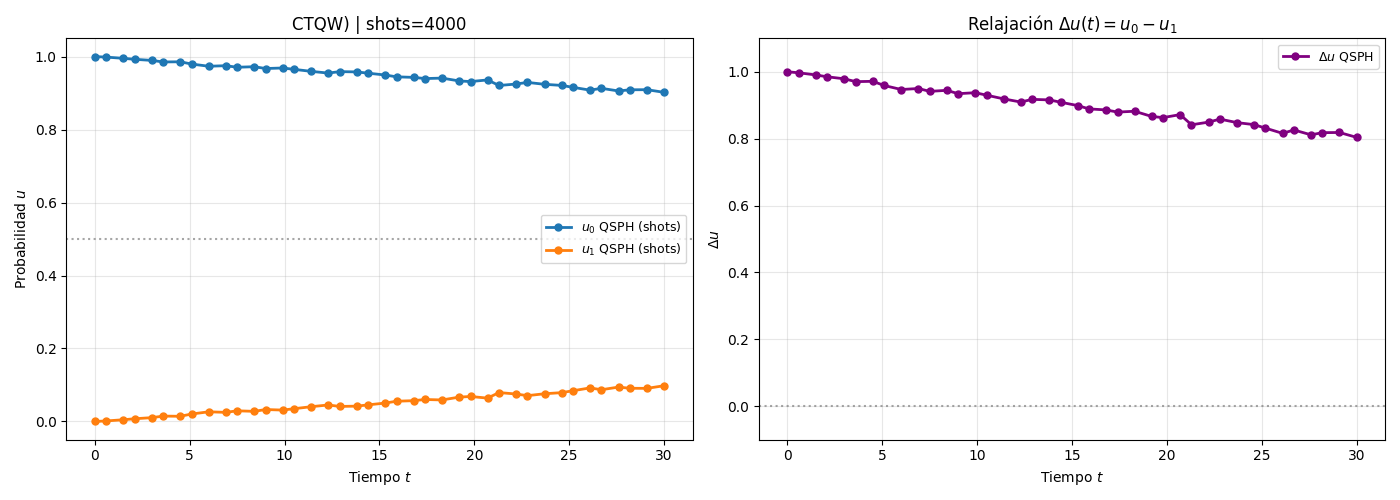
\includegraphics[width=0.95\textwidth]{chapters/cap5_circuito/img/sim_con_medida_inter.png}
    \caption{Evolución de las probabilidades del sistema tras introducir la interacción con el ancilla, la medición intermedia y el reinicio condicional. El patrón unitario se modifica, pero no aparece la relajación clásica.}
    \label{fig:sim-con-medida-inter}
\end{figure}

El circuito de un paso se muestra en la figura~\ref{fig:circ-medida-inter}, la cual consiste en el bloque de Matching Decomposition, $CX$ hacia el ancilla, medición intermedia y, si procede, $X$ de reinicio.

\begin{figure}[htbp]
    \centering
    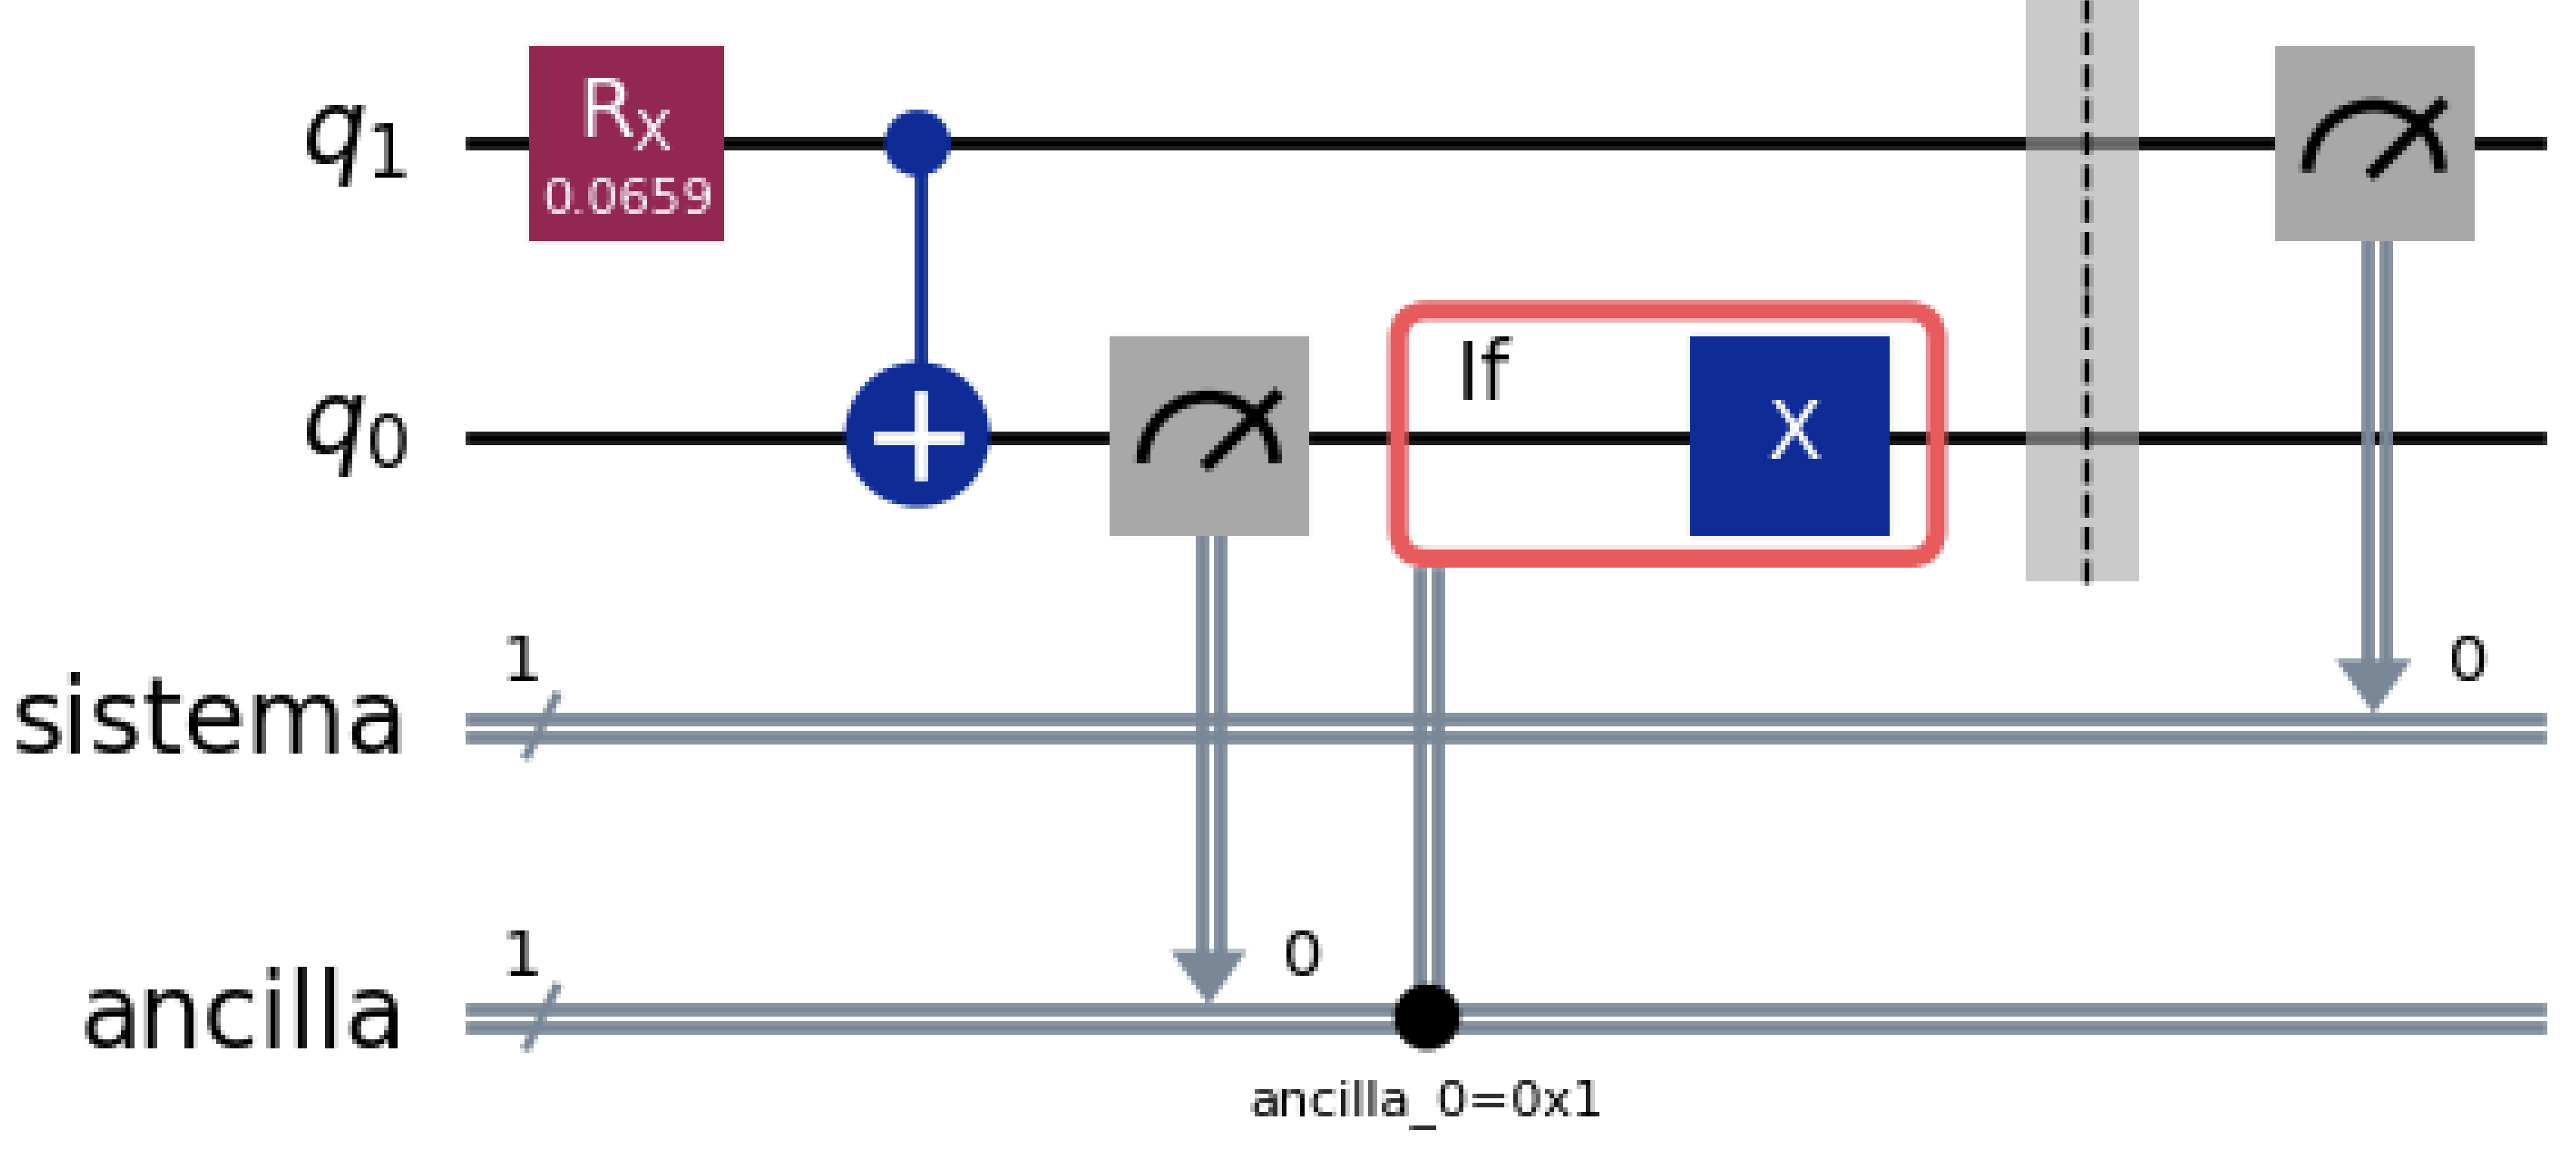
\includegraphics[width=\textwidth]{chapters/cap5_circuito/img/circ_medidainter.png}
    \caption{Circuito de un paso de Trotter con interacción sistema--ancilla, medición intermedia y reinicio condicional del ancilla.}
    \label{fig:circ-medida-inter}
\end{figure}

\section{Compensación del efecto Zeno}
\label{sec:compensacion-zeno}

La medición del ancilla en cada paso de Trotter no es neutra. Además de abrir el sistema, interrumpe la evolución coherente y puede reducir, o incluso congelar, la transferencia de amplitud entre partículas. Ese fenómeno es el efecto Zeno cuántico~\cite{nielsen2010,Kondo2016QZE}.

Para un sistema de dos niveles que parte de $\ket{0}$, un acoplamiento $J_{\mathrm{eff}}$ produce, en un intervalo $\Delta t$ y \emph{antes} de medir, la probabilidad de ocupación del segundo nodo~\cite{nielsen2010}
\begin{equation}
    P_{1}(\Delta t)
    =
    \sin^{2}\bigl(J_{\mathrm{eff}}\Delta t\bigr).
    \label{eq:probabilidad-transferencia-zeno}
\end{equation}
En el circuito cerrado esa expresión es la transferencia neta por paso. En el circuito abierto, la $CX$ y la medida del ancilla cortan esa evolución. Si $\Delta t$ es demasiado pequeño frente a $1/\Vert J\Vert$, el sistema apenas abandona $\ket{0}$ y la cantidad advectada queda prácticamente congelada~\cite{Kondo2016QZE}. Esa es la razón por la que la figura~\ref{fig:sim-con-medida-inter} no reproduce la relajación clásica de la figura~\ref{fig:cassical_sim}.

La compensación consiste en elegir $J_{\mathrm{eff}}$ de modo que la expresión \eqref{eq:probabilidad-transferencia-zeno} coincida con la probabilidad de transferencia del paso de Euler SPH. Si $J_{\mathrm{classic}}$ es el coeficiente de la matriz hermítica $J$, detallada en la sección \ref{sec:primera_implementacion}, se impone lo siguiente:

\begin{equation}
    \sin^{2}\bigl(J_{\mathrm{eff}}\Delta t\bigr)
    =
    J_{\mathrm{classic}}\Delta t,
    \label{eq:condicion-compensacion-zeno}
\end{equation}
de donde
\begin{equation}
    J_{\mathrm{eff}}
    =
    \frac{\arcsin\bigl(\sqrt{J_{\mathrm{classic}}\Delta t}\bigr)}{\Delta t},
    \qquad
    0\leq J_{\mathrm{classic}}\Delta t\leq 1.
    \label{eq:J-eff}
\end{equation}
La cota $J_{\mathrm{classic}}\Delta t\leq 1$ garantiza que el argumento de la raíz sea una probabilidad. Si se viola, hay que reducir $\Delta t$ aumentando el número de pasos de Trotter.

La expresión~\eqref{eq:J-eff} no aparece en la literatura de QSPH ni en los trabajos de Zeno citados, se trata de una calibración introducida en este trabajo. Lo que sí está en la literatura es el mecanismo que se corrige. La dependencia $\sin^{2}$ es la evolución unitaria de un sistema de dos niveles~\cite{nielsen2010}. La inhibición de esa evolución al medir con frecuencia es el efecto Zeno~\cite{Kondo2016QZE,Misra1977QZE}. La transformación $J\rightarrow J_{\mathrm{eff}}$ invierte localmente esa dependencia sinusoidal para que, una vez medida el ancilla, el salto por paso recupere la tasa clásica $J_{\mathrm{classic}}\Delta t$.

El hamiltoniano que entra en Matching Decomposition deja de ser la matriz $J$ de la ecuación~\eqref{mat: J} y pasa a ser
\begin{equation}
    J_{\mathrm{eff}}^{(\mathrm{mat})}
    =
    \begin{pmatrix}
        0 & J_{\mathrm{eff}}\\
        J_{\mathrm{eff}} & 0
    \end{pmatrix}.
    \label{eq:J-eff-matrix}
\end{equation}
La topología no cambia, sigue habiendo una única arista entre las dos partículas. Solo se reescala el acoplamiento.

Quedan, por tanto, dos piezas distintas. El ancilla, la $CX$, la medida y el reinicio abren el sistema~\cite{nielsen2010,Kondo2016QZE}. La sustitución~\eqref{eq:J-eff} no es una segunda fuente de disipación, es una corrección del acoplamiento para que el efecto Zeno no anule la tasa SPH. 

\section{Implementación final}

Con lo anterior se han definido todos los elementos necesarios para la implementación final, la evolución coherente mediante Matching Decomposition, la interacción sistema--ancilla mediante una puerta CNOT, la medición intermedia con reinicio condicional y la sustitución del acoplamiento original por el hamiltoniano efectivo $J_{\mathrm{eff}}$.

La última implementación combina estos componentes en cada paso de Trotter. Su objetivo es reproducir una transferencia compatible con la discretización clásica en el dímero $N=2$, sin mantener las oscilaciones indefinidas características del sistema cerrado. Los resultados numéricos, la comparación con la simulación clásica de la figura~\ref{fig:cassical_sim} y el análisis de la influencia de la frecuencia de medida se presentan en el capítulo~\ref{cap:resultados}.


% chapters/cap6_resultados/cap6.tex

\chapter{Resultados y Discusión}
\label{cap:resultados}

Este capítulo contrasta la relajación del dímero SPH~\eqref{eq:sph_advection_discrete} con el circuito abierto descrito en el capítulo~\ref{cap:implementacion_circuito}. En todos los ensayos cuánticos se emplearon $4000$ lanzamientos. Los parámetros físicos son los mismos que los puestos en el capítulo~\ref{cap:metodologia}.
\section{Referencia clásica y simulación cuántica}

La referencia clásica se construye con la ecuación de advección discreta~\eqref{eq:sph_advection_discrete}. Ese esquema es recursivo ya que el estado en $t_0+\Delta t$ exige conocer el estado en $t_0$. Cada incremento temporal reutiliza las cantidades $u_j(t_0)$ de ambas partículas, de forma que el detalle de la trayectoria depende de $\Delta t$, mientras se reduce este valor mejor es el detalle y por ende, el comportamiento se apega más a la realidad. El resultado se muestra en la figura~\ref{fig:cassical_sim}.

\begin{figure}[htbp]
    \centering
    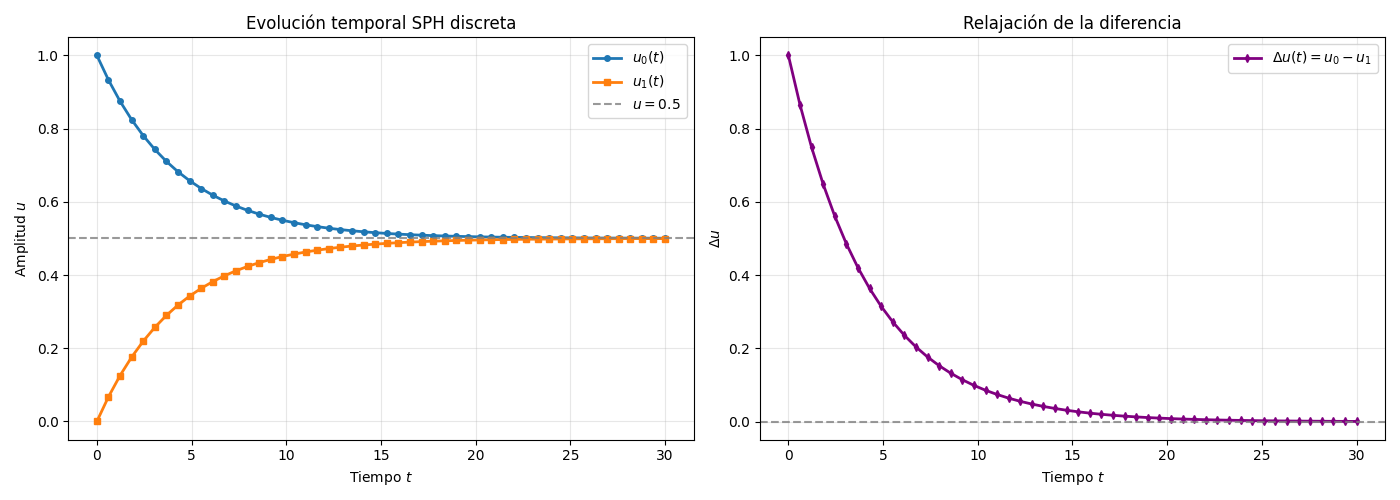
\includegraphics[width=0.95\textwidth]{chapters/cap6_resultados/img/clasical.png}
    \caption{Simulación clásica de dos partículas con la discretización SPH~\eqref{eq:sph_advection_discrete}.}
    \label{fig:cassical_sim}
\end{figure}

La simulación cuántica emplea el mismo escenario: dos partículas, la misma condición inicial y los mismos parámetros. El bloque elemental es el de la figura~\ref{fig:circ-medida-inter}, repetido $100$ veces. Las curvas cuánticas corresponden a las poblaciones $P_j = \rho_{jj}$, identificadas con $u_j$ como se indicó en la sección~\ref{sec:codificacion_estado}. Para reconstruir la curva se muestrearon $40$ instantes uniformes entre $t=0$ y $t=30$. El resultado aparece en la figura~\ref{fig:sim_definitive}. Ambas evoluciones son comparables: la cantidad advectada abandona la partícula $0$, se transfiere a la partícula $1$ y se aproxima al equilibrio en $0{,}5$, sin el rebote sinusoidal del circuito cerrado. Ese equilibrio es el de la ODE~\eqref{eq:sph_advection_discrete} con partículas fijas.

\begin{figure}[htbp]
    \centering
    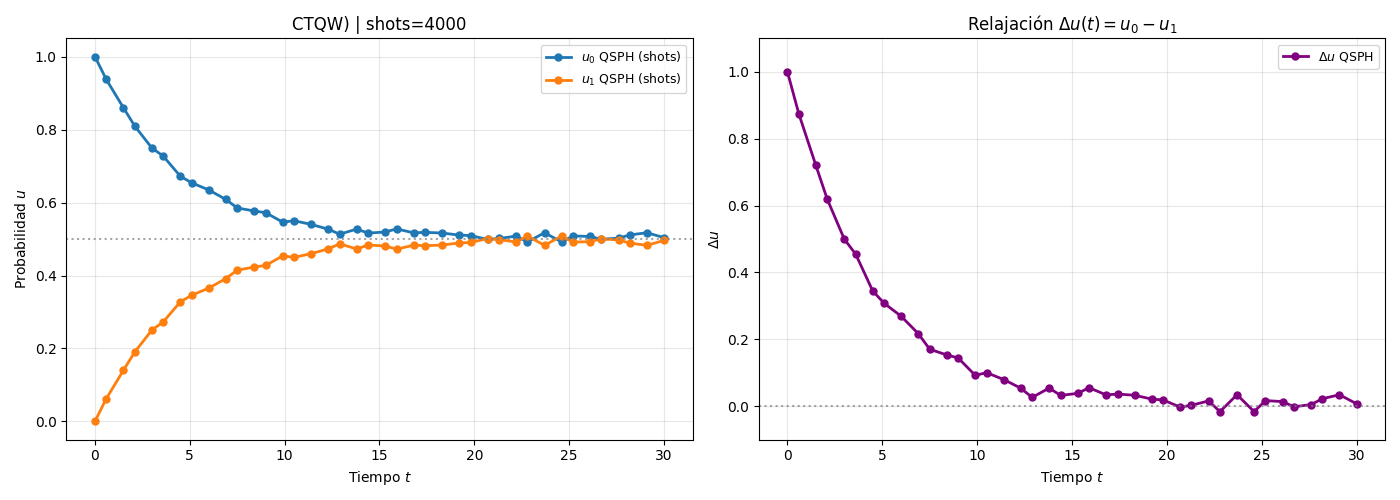
\includegraphics[width=0.95\textwidth]{chapters/cap6_resultados/img/cuantum-sim.png}
    \caption{Simulación cuántica con Hamiltoniano efectivo, ancilla y medición intermedia. Se muestran las poblaciones $P_j$, identificadas con $u_j$, y $40$ instantes para comparar el comportamiento con la referencia clásica.}
    \label{fig:sim_definitive}
\end{figure}

\section{Lectura del estado inicial y final}

La figura~\ref{fig:sim_definitive} sirve para comparar trayectorias. No es, sin embargo, un requisito del algoritmo cuántico. El esquema clásico no puede saltar de $t=0$ a $t=30$ sin calcular los estados intermedios. En cambio el algoritmo cuántico sí, basta concatenar los $100$ bloques de la figura~\ref{fig:circ-medida-inter} y medir el qubit del sistema al final. La figura~\ref{fig:ventaja} muestra únicamente esos dos extremos. El estado inicial y el estado a $t=30$ coinciden con los de la curva completa, sin recorrer el camino punto a punto.

\begin{figure}[htbp]
    \centering
    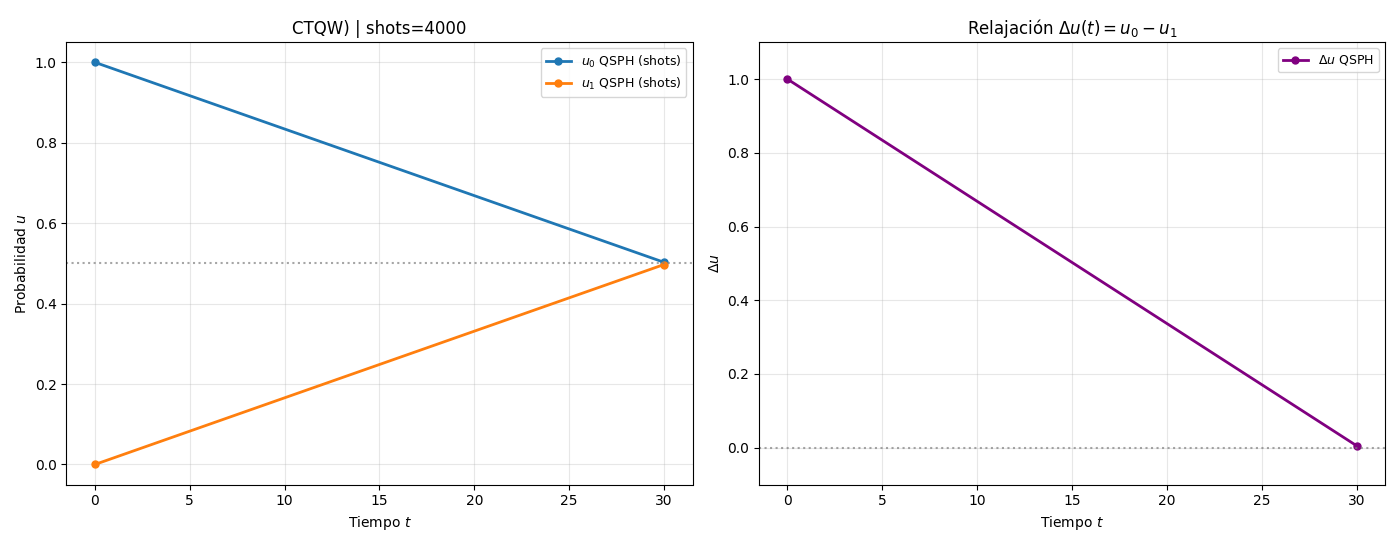
\includegraphics[width=0.95\textwidth]{chapters/cap6_resultados/img/ventaja.png}
    \caption{Lectura directa del estado inicial y del estado a $t=30$ tras aplicar $100$ bloques de Trotter, sin reconstruir la trayectoria intermedia.}
    \label{fig:ventaja}
\end{figure}

\begin{figure}[htbp]
    \centering
    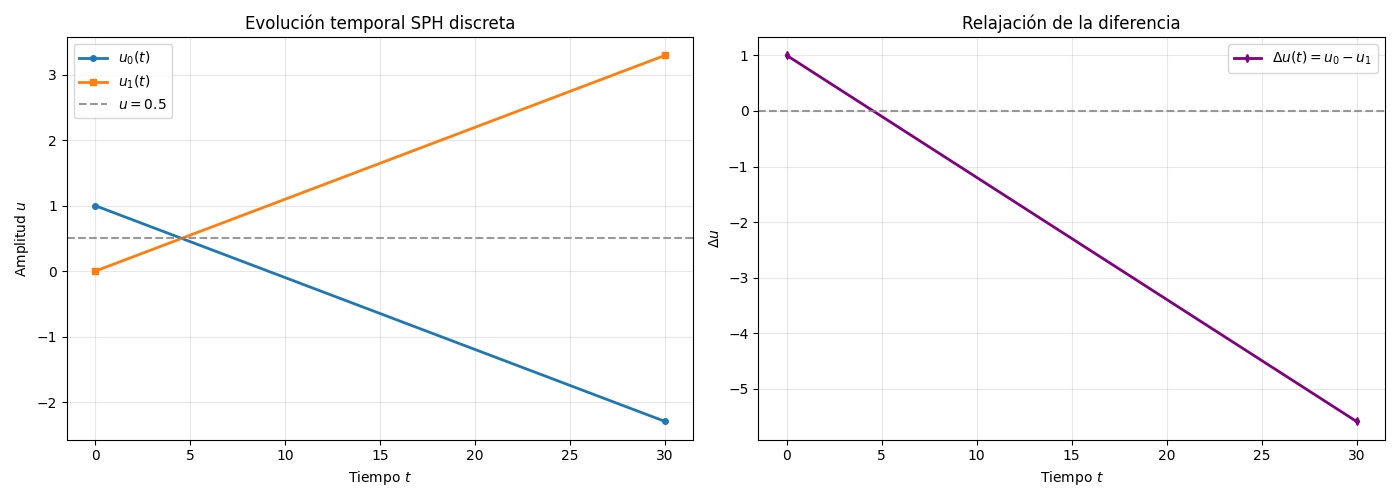
\includegraphics[width=0.95\textwidth]{chapters/cap6_resultados/img/classic-0-a-30-un-paso.png}
    \caption{Lectura directa del estado inicial y del estado a $t=30$ con simulación clásica}
    \label{fig:ventaja_classic}
\end{figure}

Esta diferencia es operativa. La gráfica de $40$ puntos se usó solo para validar el comportamiento. Una vez aceptada la correspondencia con la ecuación (\eqref{eq:sph_advection_discrete}), el circuito puede ejecutarse de una vez sobre el intervalo completo y devolver la cantidad advectada final. Es una diferencia de este circuito de Trotter concatenado frente al Euler recursivo en $N=2$, no una demostración de \emph{speedup} asintótico.

\section{Variación de la velocidad de advección}

Como comprobación adicional se realizarón más pruebas variando la velocidad de advección $c$ de $10^{-0{,}5}$ a $10^{-1}$ y $10^{-0.2}$, manteniendo el resto de parámetros. Disminuir $c$ debilita el acoplamiento entre partículas, en la misma dirección que los ensayos de ~\cite{auyeung2025}, donde una menor interacción retrasa el transporte de la cantidad advectada. Las figuras~\ref{fig:clasico-c-menor} y~\ref{fig:cuantico-c-menor} muestran el caso clásico y el cuántico. A $t=30$ el sistema ya no alcanza el equilibrio en $0{,}5$: la transferencia es más lenta y ambas descripciones vuelven a coincidir. 

Por otro lado el hecho de aumentar $c$ aumenta la fuerza de acoplamiento haciendo que la interacción y relajación suceda de forma más rápida, tal como se ve en \ref{fig:clasico-c-mayor} y en \ref{fig:cuantico-c-mayor}. El circuito sigue, por tanto, la relajación de la ecuación~\eqref{eq:sph_advection_discrete} al variar $c$.

\begin{figure}[htbp]
    \centering
    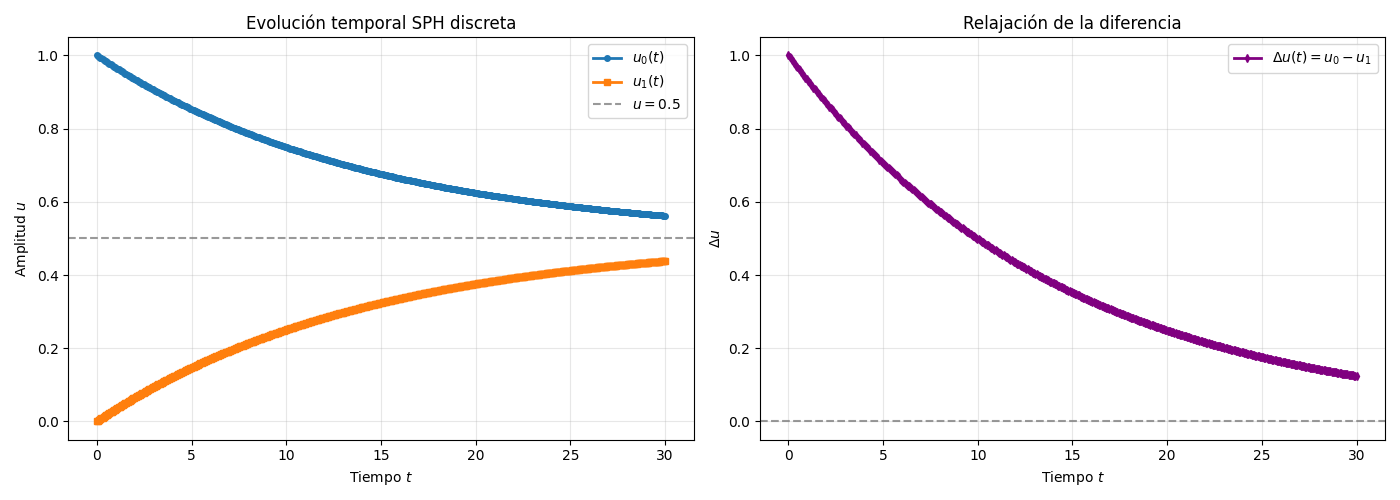
\includegraphics[width=0.95\textwidth]{chapters/cap6_resultados/img/cla-c-menor.png}
    \caption{Simulación clásica con $c=10^{-1}$.}
    \label{fig:clasico-c-menor}
\end{figure}

\begin{figure}[htbp]
    \centering
    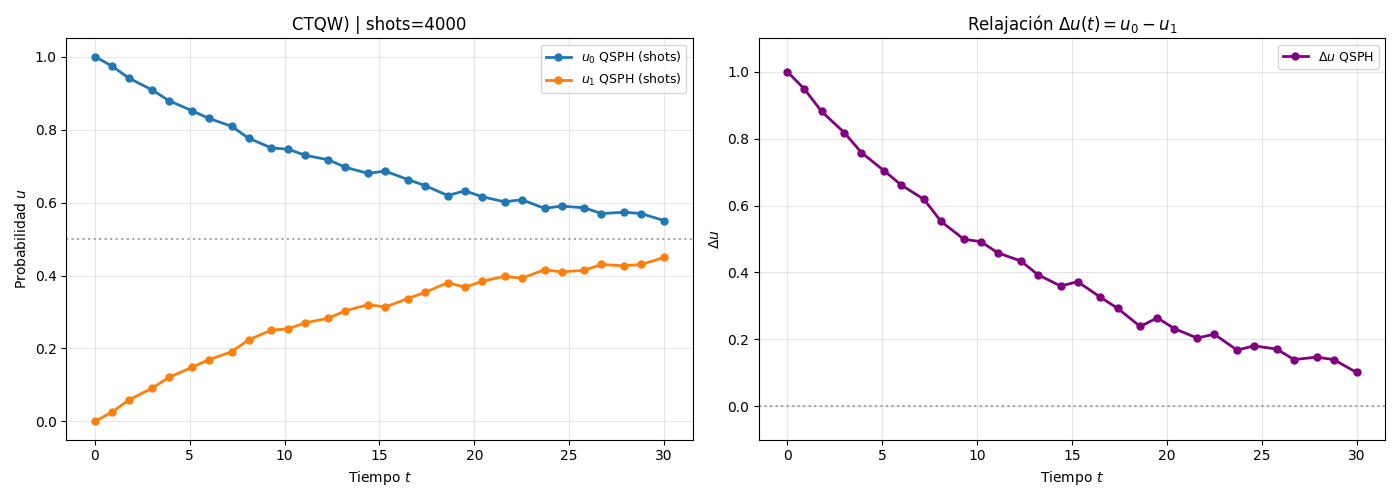
\includegraphics[width=0.95\textwidth]{chapters/cap6_resultados/img/cua-c-menor.png}
    \caption{Simulación cuántica con $c=10^{-1}$.}
    \label{fig:cuantico-c-menor}
\end{figure}

\begin{figure}[htbp]
    \centering
    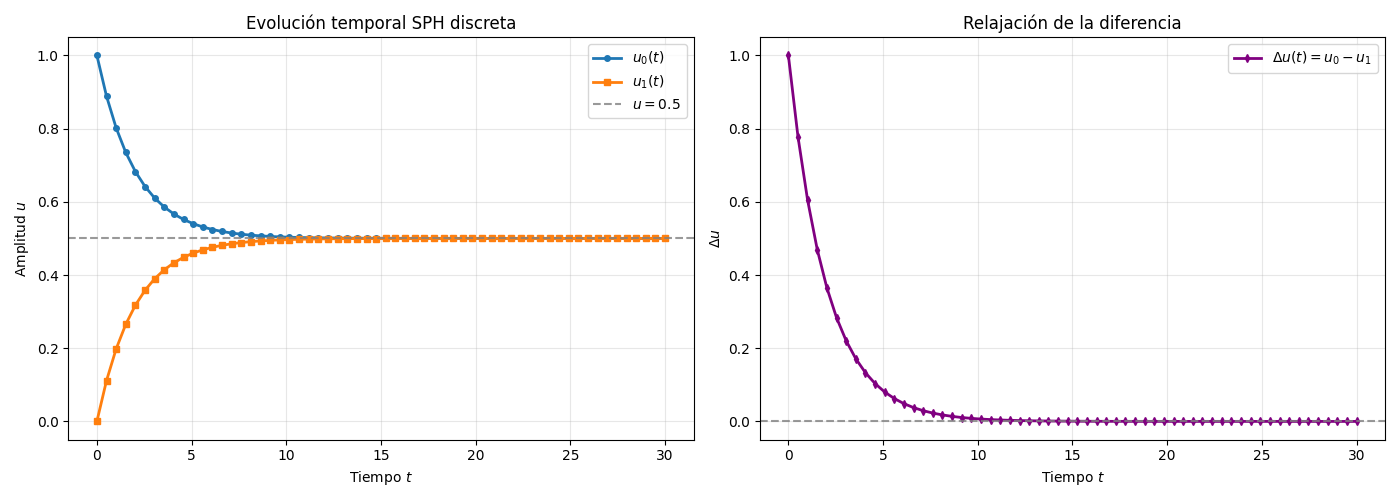
\includegraphics[width=0.95\textwidth]{chapters/cap6_resultados/img/cla-c-mayor.png}
    \caption{Simulación cuántica con $c=10^{-0.2}$.}
    \label{fig:cuantico-c-mayor}
\end{figure}

\begin{figure}[htbp]
    \centering
    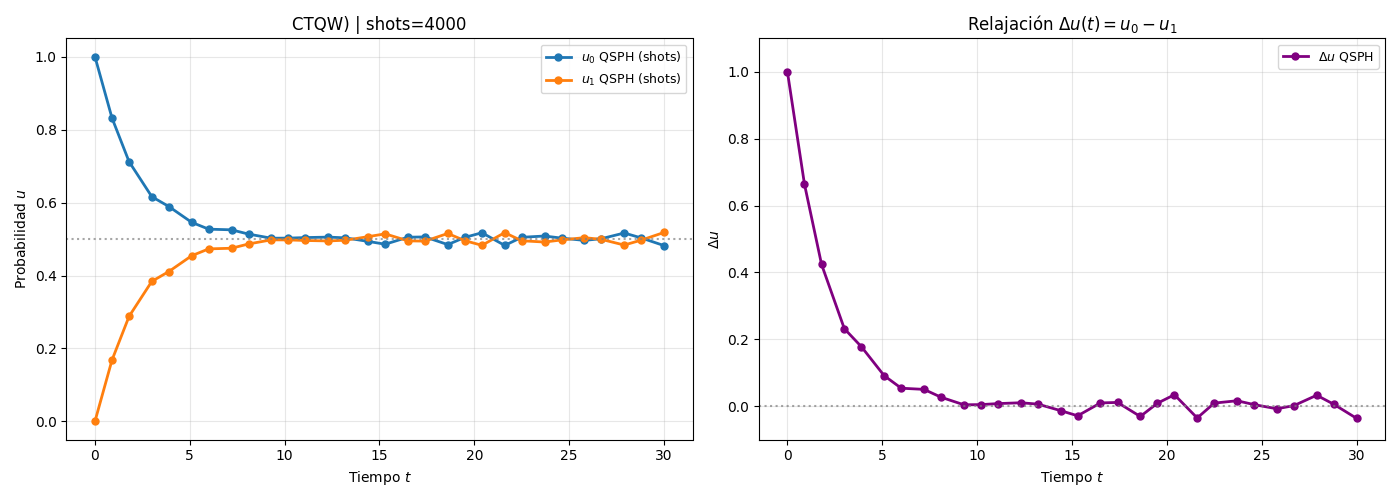
\includegraphics[width=0.95\textwidth]{chapters/cap6_resultados/img/cua-c-mayor.png}
    \caption{Simulación cuántica con $c=10^{-0.2}$.}
    \label{fig:clasico-c-mayor}
\end{figure}

% chapters/cap7_conclusiones/cap7.tex

\chapter{Conclusiones y Trabajo Futuro}
\label{sec:conclusiones}

\section{Conclusiones}

Este trabajo diseñó, implementó y evaluó un algoritmo de \emph{Quantum Smoothed Particle Hydrodynamics} (QSPH) basado en \emph{Continuous-Time Quantum Walks} (CTQW) para la ecuación de advección unidimensional, dando así respuesta al objetivo general planteado en el capítulo~\ref{ch:objetivos}. En el caso de dos partículas, el circuito abierto ---\emph{Matching Decomposition} (sección~\ref{sec:matching_decomposition}), qubit ancilla y medición intermedia con reinicio como modelo de colisión~\cite{Ciccarello_2022} (sección~\ref{sec:implementacion-ancilla}), y hamiltoniano efectivo $J_{\mathrm{eff}}$ (ecuación~\eqref{eq:J-eff}) que compensa el efecto Zeno (sección~\ref{sec:compensacion-zeno})--- reproduce la transferencia y el equilibrio de la discretización SPH clásica~\eqref{eq:sph_advection_discrete}, tanto para $c=10^{-0{,}5}$ (figura~\ref{fig:sim_definitive}) como para $c=10^{-1}$ (figura~\ref{fig:cuantico-c-menor}).

La primera conclusión de diseño es que el CTQW cerrado no basta. El operador $\hat{U}(t)=e^{-iJt}$ (ecuación~\eqref{eq:operador_U_ctqw}) conserva la energía y genera un intercambio periódico de la cantidad advectada ---las oscilaciones sinusoidales de la figura~\ref{fig:resultado_1}--- incompatible con el atractor de la ecuación~\eqref{eq:sph_advection_discrete} en el dímero (sección~\ref{sec:primera_implementacion}). La referencia clásica, en cambio, relaja hacia $u=1/2$ porque en este caso mínimo las dos partículas permanecen fijas dentro del soporte del kernel (ecuación~\eqref{eq:sph_advection_discrete}). La analogía topológica entre el kernel SPH y la matriz de adyacencia sí es válida para construir $H$ (sección~\ref{subsec: analogía}), pero la relajación de la ecuación~\eqref{eq:sph_advection_discrete} solo aparece al abrir el sistema.

Dentro de ese alcance, el esquema presenta ventajas operativas ya discutidas en los capítulos~\ref{cap:implementacion_circuito} y~\ref{cap:resultados}. \emph{Matching Decomposition} evita la descomposición de Pauli y, en dos partículas, reduce cada paso de Trotter a una única rotación $R_x$ (ecuación~\eqref{eq:puerta_rx}), esa $R_x$ es el \emph{matching} trivial del dímero, no la eficiencia reportada por \cite{matching2026}. La lectura compara las poblaciones $P_j$ con los $u_j$ clásicos, como se definió en la sección~\ref{sec:codificacion_estado}. A diferencia del Euler clásico, que es recursivo y exige todos los estados intermedios, el circuito puede concatenar los $r$ bloques y medir únicamente el estado final, como ilustra la figura~\ref{fig:ventaja}.

La validación, no obstante, se limita a $N=2$. No se han realizado ensayos con más partículas. La construcción actual organiza la evolución en bloques de emparejamiento (sección~\ref{sec:matching_decomposition}), de modo que no cubre un número impar de nodos. Tampoco está demostrado que el protocolo abierto escale sin un ancilla y una medida \emph{mid-circuit} por cada par (sección~\ref{sec:implementacion-ancilla}), esa sobrecarga podría erosionar la eficiencia y aún no se ha cuantificado. Por tanto, el algoritmo se considera válido para analizar un sistema de dos partículas SPH junto con las resstricciones impuestas en este trabajo, y no una formulación general de QSPH.

En conjunto, el trabajo aporta una primera implementación CTQW de QSPH, compacta y físicamente coherente en el caso mínimo, pensada como base para un desarrollo futuro.

\section{Líneas de trabajo futuro}

El paso más lógico e inmediato es generalizar el algoritmo. Hay que aprovechar el \emph{matching} (sección~\ref{sec:matching_decomposition}), la codificación de amplitudes y el mapa de Lindblad~\eqref{eq:lindblad} para $N>2$ y comprobar si cada par requiere su propio ancilla y su propia medida intermedia (sección~\ref{sec:implementacion-ancilla}). Esas pruebas dirán si el canal de colisión sigue reproduciendo la relajación de la ecuación~\eqref{eq:sph_advection_discrete} o si el efecto Zeno (sección~\ref{sec:compensacion-zeno}) y el recuento de qubits vuelven el circuito inviable. Como validación futura conviene, además, introducir una métrica cuantitativa (por ejemplo, el error $L^2$ frente a la solución de la ecuación~\eqref{eq:sph_advection_discrete}) y ensayar un caso $N=4$, donde el \emph{matching} deja de ser trivial.

En paralelo conviene anclar la propuesta al hardware real, en el caso de que los bloques se hagan extensos habra que valorar el reducir profundidad, tolerar ruido, tomar en cuenta las conecciones y restricciones de cada computador y medir fidelidad fuera del simulador ideal. El objetivo a medio plazo no es sustituir ya al SPH clásico, sino dejar un QSPH robusto, accesible y, cuando existan procesadores más capaces, competitivo en tiempo con la integración explícita convencional.


% ─── BACKMATTER ───────────────────────────────────────────────────────────────
\backmatter
\pagenumbering{bychapter}

% Índice analítico
\printindex

% Bibliografía
\bibliography{referencias}

\end{document}
